%% bare_adv.tex
%% V1.4b
%% 2015/08/26
%% by Michael Shell
%% See: 
%% http://www.michaelshell.org/
%% for current contact information.
%%
%% This is a skeleton file demonstrating the advanced use of IEEEtran.cls
%% (requires IEEEtran.cls version 1.8b or later) with an IEEE Computer
%% Society journal paper.
%%
%% Support sites:
%% http://www.michaelshell.org/tex/ieeetran/
%% http://www.ctan.org/pkg/ieeetran
%% and
%% http://www.ieee.org/

%%*************************************************************************
%% Legal Notice:
%% This code is offered as-is without any warranty either expressed or
%% implied; without even the implied warranty of MERCHANTABILITY or
%% FITNESS FOR A PARTICULAR PURPOSE! 
%% User assumes all risk.
%% In no event shall the IEEE or any contributor to this code be liable for
%% any damages or losses, including, but not limited to, incidental,
%% consequential, or any other damages, resulting from the use or misuse
%% of any information contained here.
%%
%% All comments are the opinions of their respective authors and are not
%% necessarily endorsed by the IEEE.
%%
%% This work is distributed under the LaTeX Project Public License (LPPL)
%% ( http://www.latex-project.org/ ) version 1.3, and may be freely used,
%% distributed and modified. A copy of the LPPL, version 1.3, is included
%% in the base LaTeX documentation of all distributions of LaTeX released
%% 2003/12/01 or later.
%% Retain all contribution notices and credits.
%% ** Modified files should be clearly indicated as such, including  **
%% ** renaming them and changing author support contact information. **
%%*************************************************************************


% *** Authors should verify (and, if needed, correct) their LaTeX system  ***
% *** with the testflow diagnostic prior to trusting their LaTeX platform ***
% *** with production work. The IEEE's font choices and paper sizes can   ***
% *** trigger bugs that do not appear when using other class files.       ***                          ***
% The testflow support page is at:
% http://www.michaelshell.org/tex/testflow/




% IEEEtran V1.7 and later provides for these CLASSINPUT macros to allow the
% user to reprogram some IEEEtran.cls defaults if needed. These settings
% override the internal defaults of IEEEtran.cls regardless of which class
% options are used. Do not use these unless you have good reason to do so as
% they can result in nonIEEE compliant documents. User beware. ;)
%
%\newcommand{\CLASSINPUTbaselinestretch}{1.0} % baselinestretch
%\newcommand{\CLASSINPUTinnersidemargin}{1in} % inner side margin
%\newcommand{\CLASSINPUToutersidemargin}{1in} % outer side margin
%\newcommand{\CLASSINPUTtoptextmargin}{1in}   % top text margin
%\newcommand{\CLASSINPUTbottomtextmargin}{1in}% bottom text margin




%
\documentclass[10pt,journal,compsoc]{IEEEtran}
% If IEEEtran.cls has not been installed into the LaTeX system files,
% manually specify the path to it like:
% \documentclass[10pt,journal,compsoc]{../sty/IEEEtran}


% For Computer Society journals, IEEEtran defaults to the use of 
% Palatino/Palladio as is done in IEEE Computer Society journals.
% To go back to Times Roman, you can use this code:
%\renewcommand{\rmdefault}{ptm}\selectfont





% Some very useful LaTeX packages include:
% (uncomment the ones you want to load)



% *** MISC UTILITY PACKAGES ***
%
%\usepackage{ifpdf}
% Heiko Oberdiek's ifpdf.sty is very useful if you need conditional
% compilation based on whether the output is pdf or dvi.
% usage:
% \ifpdf
%   % pdf code
% \else
%   % dvi code
% \fi
% The latest version of ifpdf.sty can be obtained from:
% http://www.ctan.org/pkg/ifpdf
% Also, note that IEEEtran.cls V1.7 and later provides a builtin
% \ifCLASSINFOpdf conditional that works the same way.
% When switching from latex to pdflatex and vice-versa, the compiler may
% have to be run twice to clear warning/error messages.






% *** CITATION PACKAGES ***
%
\ifCLASSOPTIONcompsoc
  % The IEEE Computer Society needs nocompress option
  % requires cite.sty v4.0 or later (November 2003)
  \usepackage[nocompress]{cite}
\else
  % normal IEEE
  \usepackage{cite}
\fi
% cite.sty was written by Donald Arseneau
% V1.6 and later of IEEEtran pre-defines the format of the cite.sty package
% \cite{} output to follow that of the IEEE. Loading the cite package will
% result in citation numbers being automatically sorted and properly
% "compressed/ranged". e.g., [1], [9], [2], [7], [5], [6] without using
% cite.sty will become [1], [2], [5]--[7], [9] using cite.sty. cite.sty's
% \cite will automatically add leading space, if needed. Use cite.sty's
% noadjust option (cite.sty V3.8 and later) if you want to turn this off
% such as if a citation ever needs to be enclosed in parenthesis.
% cite.sty is already installed on most LaTeX systems. Be sure and use
% version 5.0 (2009-03-20) and later if using hyperref.sty.
% The latest version can be obtained at:
% http://www.ctan.org/pkg/cite
% The documentation is contained in the cite.sty file itself.
%
% Note that some packages require special options to format as the Computer
% Society requires. In particular, Computer Society  papers do not use
% compressed citation ranges as is done in typical IEEE papers
% (e.g., [1]-[4]). Instead, they list every citation separately in order
% (e.g., [1], [2], [3], [4]). To get the latter we need to load the cite
% package with the nocompress option which is supported by cite.sty v4.0
% and later.





% *** GRAPHICS RELATED PACKAGES ***
%
\ifCLASSINFOpdf
  % \usepackage[pdftex]{graphicx}
  % declare the path(s) where your graphic files are
  % \graphicspath{{../pdf/}{../jpeg/}}
  % and their extensions so you won't have to specify these with
  % every instance of \includegraphics
  % \DeclareGraphicsExtensions{.pdf,.jpeg,.png}
\else
  % or other class option (dvipsone, dvipdf, if not using dvips). graphicx
  % will default to the driver specified in the system graphics.cfg if no
  % driver is specified.
  % \usepackage[dvips]{graphicx}
  % declare the path(s) where your graphic files are
  % \graphicspath{{../eps/}}
  % and their extensions so you won't have to specify these with
  % every instance of \includegraphics
  % \DeclareGraphicsExtensions{.eps}
\fi
% graphicx was written by David Carlisle and Sebastian Rahtz. It is
% required if you want graphics, photos, etc. graphicx.sty is already
% installed on most LaTeX systems. The latest version and documentation
% can be obtained at: 
% http://www.ctan.org/pkg/graphicx
% Another good source of documentation is "Using Imported Graphics in
% LaTeX2e" by Keith Reckdahl which can be found at:
% http://www.ctan.org/pkg/epslatex
%
% latex, and pdflatex in dvi mode, support graphics in encapsulated
% postscript (.eps) format. pdflatex in pdf mode supports graphics
% in .pdf, .jpeg, .png and .mps (metapost) formats. Users should ensure
% that all non-photo figures use a vector format (.eps, .pdf, .mps) and
% not a bitmapped formats (.jpeg, .png). The IEEE frowns on bitmapped formats
% which can result in "jaggedy"/blurry rendering of lines and letters as
% well as large increases in file sizes.
%
% You can find documentation about the pdfTeX application at:
% http://www.tug.org/applications/pdftex





% *** MATH PACKAGES ***
%
\usepackage{amsmath}
\usepackage{cite}
\usepackage{multirow}
\usepackage{graphicx}
\usepackage{amsfonts}
\usepackage[T1]{fontenc}
\usepackage{algorithmic}
\usepackage{array}
\usepackage{url}
\usepackage{enumitem}
\usepackage{stfloats}
\usepackage{float}
\usepackage{caption}
\usepackage{subcaption}
\usepackage{mathtools}
\DeclarePairedDelimiter\ceil{\lceil}{\rceil}
\DeclarePairedDelimiter\floor{\lfloor}{\rfloor}

% A popular package from the American Mathematical Society that provides
% many useful and powerful commands for dealing with mathematics.
%
% Note that the amsmath package sets \interdisplaylinepenalty to 10000
% thus preventing page breaks from occurring within multiline equations. Use:
%\interdisplaylinepenalty=2500
% after loading amsmath to restore such page breaks as IEEEtran.cls normally
% does. amsmath.sty is already installed on most LaTeX systems. The latest
% version and documentation can be obtained at:
% http://www.ctan.org/pkg/amsmath





% *** SPECIALIZED LIST PACKAGES ***
%\usepackage{acronym}
% acronym.sty was written by Tobias Oetiker. This package provides tools for
% managing documents with large numbers of acronyms. (You don't *have* to
% use this package - unless you have a lot of acronyms, you may feel that
% such package management of them is bit of an overkill.)
% Do note that the acronym environment (which lists acronyms) will have a
% problem when used under IEEEtran.cls because acronym.sty relies on the
% description list environment - which IEEEtran.cls has customized for
% producing IEEE style lists. A workaround is to declared the longest
% label width via the IEEEtran.cls \IEEEiedlistdecl global control:
%
% \renewcommand{\IEEEiedlistdecl}{\IEEEsetlabelwidth{SONET}}
% \begin{acronym}
%
% \end{acronym}
% \renewcommand{\IEEEiedlistdecl}{\relax}% remember to reset \IEEEiedlistdecl
%
% instead of using the acronym environment's optional argument.
% The latest version and documentation can be obtained at:
% http://www.ctan.org/pkg/acronym


%\usepackage{algorithmic}
\usepackage[linesnumbered,lined,boxed,commentsnumbered]{algorithm2e}
% algorithmic.sty was written by Peter Williams and Rogerio Brito.
% This package provides an algorithmic environment fo describing algorithms.
% You can use the algorithmic environment in-text or within a figure
% environment to provide for a floating algorithm. Do NOT use the algorithm
% floating environment provided by algorithm.sty (by the same authors) or
% algorithm2e.sty (by Christophe Fiorio) as the IEEE does not use dedicated
% algorithm float types and packages that provide these will not provide
% correct IEEE style captions. The latest version and documentation of
% algorithmic.sty can be obtained at:
% http://www.ctan.org/pkg/algorithms
% Also of interest may be the (relatively newer and more customizable)
% algorithmicx.sty package by Szasz Janos:
% http://www.ctan.org/pkg/algorithmicx




% *** ALIGNMENT PACKAGES ***
%
%\usepackage{array}
% Frank Mittelbach's and David Carlisle's array.sty patches and improves
% the standard LaTeX2e array and tabular environments to provide better
% appearance and additional user controls. As the default LaTeX2e table
% generation code is lacking to the point of almost being broken with
% respect to the quality of the end results, all users are strongly
% advised to use an enhanced (at the very least that provided by array.sty)
% set of table tools. array.sty is already installed on most systems. The
% latest version and documentation can be obtained at:
% http://www.ctan.org/pkg/array


%\usepackage{mdwmath}
%\usepackage{mdwtab}
% Also highly recommended is Mark Wooding's extremely powerful MDW tools,
% especially mdwmath.sty and mdwtab.sty which are used to format equations
% and tables, respectively. The MDWtools set is already installed on most
% LaTeX systems. The lastest version and documentation is available at:
% http://www.ctan.org/pkg/mdwtools


% IEEEtran contains the IEEEeqnarray family of commands that can be used to
% generate multiline equations as well as matrices, tables, etc., of high
% quality.


%\usepackage{eqparbox}
% Also of notable interest is Scott Pakin's eqparbox package for creating
% (automatically sized) equal width boxes - aka "natural width parboxes".
% Available at:
% http://www.ctan.org/pkg/eqparbox




% *** SUBFIGURE PACKAGES ***
%\ifCLASSOPTIONcompsoc
%  \usepackage[caption=false,font=footnotesize,labelfont=sf,textfont=sf]{subfig}
%\else
%  \usepackage[caption=false,font=footnotesize]{subfig}
%\fi
% subfig.sty, written by Steven Douglas Cochran, is the modern replacement
% for subfigure.sty, the latter of which is no longer maintained and is
% incompatible with some LaTeX packages including fixltx2e. However,
% subfig.sty requires and automatically loads Axel Sommerfeldt's caption.sty
% which will override IEEEtran.cls' handling of captions and this will result
% in non-IEEE style figure/table captions. To prevent this problem, be sure
% and invoke subfig.sty's "caption=false" package option (available since
% subfig.sty version 1.3, 2005/06/28) as this is will preserve IEEEtran.cls
% handling of captions.
% Note that the Computer Society format requires a sans serif font rather
% than the serif font used in traditional IEEE formatting and thus the need
% to invoke different subfig.sty package options depending on whether
% compsoc mode has been enabled.
%
% The latest version and documentation of subfig.sty can be obtained at:
% http://www.ctan.org/pkg/subfig




% *** FLOAT PACKAGES ***
%
%\usepackage{fixltx2e}
% fixltx2e, the successor to the earlier fix2col.sty, was written by
% Frank Mittelbach and David Carlisle. This package corrects a few problems
% in the LaTeX2e kernel, the most notable of which is that in current
% LaTeX2e releases, the ordering of single and double column floats is not
% guaranteed to be preserved. Thus, an unpatched LaTeX2e can allow a
% single column figure to be placed prior to an earlier double column
% figure.
% Be aware that LaTeX2e kernels dated 2015 and later have fixltx2e.sty's
% corrections already built into the system in which case a warning will
% be issued if an attempt is made to load fixltx2e.sty as it is no longer
% needed.
% The latest version and documentation can be found at:
% http://www.ctan.org/pkg/fixltx2e


%\usepackage{stfloats}
% stfloats.sty was written by Sigitas Tolusis. This package gives LaTeX2e
% the ability to do double column floats at the bottom of the page as well
% as the top. (e.g., "\begin{figure*}[!b]" is not normally possible in
% LaTeX2e). It also provides a command:
%\fnbelowfloat
% to enable the placement of footnotes below bottom floats (the standard
% LaTeX2e kernel puts them above bottom floats). This is an invasive package
% which rewrites many portions of the LaTeX2e float routines. It may not work
% with other packages that modify the LaTeX2e float routines. The latest
% version and documentation can be obtained at:
% http://www.ctan.org/pkg/stfloats
% Do not use the stfloats baselinefloat ability as the IEEE does not allow
% \baselineskip to stretch. Authors submitting work to the IEEE should note
% that the IEEE rarely uses double column equations and that authors should try
% to avoid such use. Do not be tempted to use the cuted.sty or midfloat.sty
% packages (also by Sigitas Tolusis) as the IEEE does not format its papers in
% such ways.
% Do not attempt to use stfloats with fixltx2e as they are incompatible.
% Instead, use Morten Hogholm'a dblfloatfix which combines the features
% of both fixltx2e and stfloats:
%
% \usepackage{dblfloatfix}
% The latest version can be found at:
% http://www.ctan.org/pkg/dblfloatfix


%\ifCLASSOPTIONcaptionsoff
%  \usepackage[nomarkers]{endfloat}
% \let\MYoriglatexcaption\caption
% \renewcommand{\caption}[2][\relax]{\MYoriglatexcaption[#2]{#2}}
%\fi
% endfloat.sty was written by James Darrell McCauley, Jeff Goldberg and 
% Axel Sommerfeldt. This package may be useful when used in conjunction with 
% IEEEtran.cls'  captionsoff option. Some IEEE journals/societies require that
% submissions have lists of figures/tables at the end of the paper and that
% figures/tables without any captions are placed on a page by themselves at
% the end of the document. If needed, the draftcls IEEEtran class option or
% \CLASSINPUTbaselinestretch interface can be used to increase the line
% spacing as well. Be sure and use the nomarkers option of endfloat to
% prevent endfloat from "marking" where the figures would have been placed
% in the text. The two hack lines of code above are a slight modification of
% that suggested by in the endfloat docs (section 8.4.1) to ensure that
% the full captions always appear in the list of figures/tables - even if
% the user used the short optional argument of \caption[]{}.
% IEEE papers do not typically make use of \caption[]'s optional argument,
% so this should not be an issue. A similar trick can be used to disable
% captions of packages such as subfig.sty that lack options to turn off
% the subcaptions:
% For subfig.sty:
% \let\MYorigsubfloat\subfloat
% \renewcommand{\subfloat}[2][\relax]{\MYorigsubfloat[]{#2}}
% However, the above trick will not work if both optional arguments of
% the \subfloat command are used. Furthermore, there needs to be a
% description of each subfigure *somewhere* and endfloat does not add
% subfigure captions to its list of figures. Thus, the best approach is to
% avoid the use of subfigure captions (many IEEE journals avoid them anyway)
% and instead reference/explain all the subfigures within the main caption.
% The latest version of endfloat.sty and its documentation can obtained at:
% http://www.ctan.org/pkg/endfloat
%
% The IEEEtran \ifCLASSOPTIONcaptionsoff conditional can also be used
% later in the document, say, to conditionally put the References on a 
% page by themselves.





% *** PDF, URL AND HYPERLINK PACKAGES ***
%
\usepackage{url}
\usepackage{hyperref}
% url.sty was written by Donald Arseneau. It provides better support for
% handling and breaking URLs. url.sty is already installed on most LaTeX
% systems. The latest version and documentation can be obtained at:
% http://www.ctan.org/pkg/url
% Basically, \url{my_url_here}.


% NOTE: PDF thumbnail features are not required in IEEE papers
%       and their use requires extra complexity and work.
%\ifCLASSINFOpdf
%  \usepackage[pdftex]{thumbpdf}
%\else
%  \usepackage[dvips]{thumbpdf}
%\fi
% thumbpdf.sty and its companion Perl utility were written by Heiko Oberdiek.
% It allows the user a way to produce PDF documents that contain fancy
% thumbnail images of each of the pages (which tools like acrobat reader can
% utilize). This is possible even when using dvi->ps->pdf workflow if the
% correct thumbpdf driver options are used. thumbpdf.sty incorporates the
% file containing the PDF thumbnail information (filename.tpm is used with
% dvips, filename.tpt is used with pdftex, where filename is the base name of
% your tex document) into the final ps or pdf output document. An external
% utility, the thumbpdf *Perl script* is needed to make these .tpm or .tpt
% thumbnail files from a .ps or .pdf version of the document (which obviously
% does not yet contain pdf thumbnails). Thus, one does a:
% 
% thumbpdf filename.pdf 
%
% to make a filename.tpt, and:
%
% thumbpdf --mode dvips filename.ps
%
% to make a filename.tpm which will then be loaded into the document by
% thumbpdf.sty the NEXT time the document is compiled (by pdflatex or
% latex->dvips->ps2pdf). Users must be careful to regenerate the .tpt and/or
% .tpm files if the main document changes and then to recompile the
% document to incorporate the revised thumbnails to ensure that thumbnails
% match the actual pages. It is easy to forget to do this!
% 
% Unix systems come with a Perl interpreter. However, MS Windows users
% will usually have to install a Perl interpreter so that the thumbpdf
% script can be run. The Ghostscript PS/PDF interpreter is also required.
% See the thumbpdf docs for details. The latest version and documentation
% can be obtained at.
% http://www.ctan.org/pkg/thumbpdf


% NOTE: PDF hyperlink and bookmark features are not required in IEEE
%       papers and their use requires extra complexity and work.
% *** IF USING HYPERREF BE SURE AND CHANGE THE EXAMPLE PDF ***
% *** TITLE/SUBJECT/AUTHOR/KEYWORDS INFO BELOW!!           ***
\newcommand\MYhyperrefoptions{bookmarks=true,bookmarksnumbered=true,
pdfpagemode={UseOutlines},plainpages=false,pdfpagelabels=true,
colorlinks=true,linkcolor={black},citecolor={black},urlcolor={black},
pdftitle={Bare Demo of IEEEtran.cls for Computer Society Journals},%<!CHANGE!
pdfsubject={Typesetting},%<!CHANGE!
pdfauthor={Michael D. Shell},%<!CHANGE!
pdfkeywords={Computer Society, IEEEtran, journal, LaTeX, paper,
             template}}%<^!CHANGE!
%\ifCLASSINFOpdf
%\usepackage[\MYhyperrefoptions,pdftex]{hyperref}
%\else
%\usepackage[\MYhyperrefoptions,breaklinks=true,dvips]{hyperref}
%\usepackage{breakurl}
%\fi
% One significant drawback of using hyperref under DVI output is that the
% LaTeX compiler cannot break URLs across lines or pages as can be done
% under pdfLaTeX's PDF output via the hyperref pdftex driver. This is
% probably the single most important capability distinction between the
% DVI and PDF output. Perhaps surprisingly, all the other PDF features
% (PDF bookmarks, thumbnails, etc.) can be preserved in
% .tex->.dvi->.ps->.pdf workflow if the respective packages/scripts are
% loaded/invoked with the correct driver options (dvips, etc.). 
% As most IEEE papers use URLs sparingly (mainly in the references), this
% may not be as big an issue as with other publications.
%
% That said, Vilar Camara Neto created his breakurl.sty package which
% permits hyperref to easily break URLs even in dvi mode.
% Note that breakurl, unlike most other packages, must be loaded
% AFTER hyperref. The latest version of breakurl and its documentation can
% be obtained at:
% http://www.ctan.org/pkg/breakurl
% breakurl.sty is not for use under pdflatex pdf mode.
%
% The advanced features offer by hyperref.sty are not required for IEEE
% submission, so users should weigh these features against the added
% complexity of use.
% The package options above demonstrate how to enable PDF bookmarks
% (a type of table of contents viewable in Acrobat Reader) as well as
% PDF document information (title, subject, author and keywords) that is
% viewable in Acrobat reader's Document_Properties menu. PDF document
% information is also used extensively to automate the cataloging of PDF
% documents. The above set of options ensures that hyperlinks will not be
% colored in the text and thus will not be visible in the printed page,
% but will be active on "mouse over". USING COLORS OR OTHER HIGHLIGHTING
% OF HYPERLINKS CAN RESULT IN DOCUMENT REJECTION BY THE IEEE, especially if
% these appear on the "printed" page. IF IN DOUBT, ASK THE RELEVANT
% SUBMISSION EDITOR. You may need to add the option hypertexnames=false if
% you used duplicate equation numbers, etc., but this should not be needed
% in normal IEEE work.
% The latest version of hyperref and its documentation can be obtained at:
% http://www.ctan.org/pkg/hyperref





% *** Do not adjust lengths that control margins, column widths, etc. ***
% *** Do not use packages that alter fonts (such as pslatex).         ***
% There should be no need to do such things with IEEEtran.cls V1.6 and later.
% (Unless specifically asked to do so by the journal or conference you plan
% to submit to, of course. )


% correct bad hyphenation here
\hyphenation{op-tical net-works semi-conduc-tor}

\newcommand{\Prob}{\mathbb{P}}
\newcommand{\Norm}{\mathcal{N}}
\newcommand{\x}{\mathbf{x}}

\begin{document}
%
% paper title
% Titles are generally capitalized except for words such as a, an, and, as,
% at, but, by, for, in, nor, of, on, or, the, to and up, which are usually
% not capitalized unless they are the first or last word of the title.
% Linebreaks \\ can be used within to get better formatting as desired.
% Do not put math or special symbols in the title.
\title{How the Gaussian Mixture Model can Fail and How to Fix it}
%
%
% author names and IEEE memberships
% note positions of commas and nonbreaking spaces ( ~ ) LaTeX will not break
% a structure at a ~ so this keeps an author's name from being broken across
% two lines.
% use \thanks{} to gain access to the first footnote area
% a separate \thanks must be used for each paragraph as LaTeX2e's \thanks
% was not built to handle multiple paragraphs
%
%
%\IEEEcompsocitemizethanks is a special \thanks that produces the bulleted
% lists the Computer Society journals use for "first footnote" author
% affiliations. Use \IEEEcompsocthanksitem which works much like \item
% for each affiliation group. When not in compsoc mode,
% \IEEEcompsocitemizethanks becomes like \thanks and
% \IEEEcompsocthanksitem becomes a line break with idention. This
% facilitates dual compilation, although admittedly the differences in the
% desired content of \author between the different types of papers makes a
% one-size-fits-all approach a daunting prospect. For instance, compsoc 
% journal papers have the author affiliations above the "Manuscript
% received ..."  text while in non-compsoc journals this is reversed. Sigh.

\author{Adam Kessler,
        Quanzhi Bi,
        Xiao Han Xiong,
        Jordan Wang,
        Yanhao Miao,
        Wanyan Shao,
        Zhaohe Huang% <-this % stops a space
% \IEEEcompsocitemizethanks{\IEEEcompsocthanksitem M. Shell was with the Department
% of Electrical and Computer Engineering, Georgia Institute of Technology, Atlanta,
% GA, 30332.\protect\\
% % note need leading \protect in front of \\ to get a newline within \thanks as
% % \\ is fragile and will error, could use \hfil\break instead.
% E-mail: see http://www.michaelshell.org/contact.html
% \IEEEcompsocthanksitem J. Doe and J. Doe are with Anonymous University.}% <-this % stops a space
\thanks{This document is the Group 2's term paper of MTH 9898, Barch College.}}

% note the % following the last \IEEEmembership and also \thanks - 
% these prevent an unwanted space from occurring between the last author name
% and the end of the author line. i.e., if you had this:
% 
% \author{....lastname \thanks{...} \thanks{...} }
%                     ^------------^------------^----Do not want these spaces!
%
% a space would be appended to the last name and could cause every name on that
% line to be shifted left slightly. This is one of those "LaTeX things". For
% instance, "\textbf{A} \textbf{B}" will typeset as "A B" not "AB". To get
% "AB" then you have to do: "\textbf{A}\textbf{B}"
% \thanks is no different in this regard, so shield the last } of each \thanks
% that ends a line with a % and do not let a space in before the next \thanks.
% Spaces after \IEEEmembership other than the last one are OK (and needed) as
% you are supposed to have spaces between the names. For what it is worth,
% this is a minor point as most people would not even notice if the said evil
% space somehow managed to creep in.



% The paper headers
\markboth{Final Project of MTH 9898: BIG DATA IN FINANCE}%
{Adam \MakeLowercase{\textit{et al.}}: How the Gaussian Mixture Model can Fail and How to Fix it}
% The only time the second header will appear is for the odd numbered pages
% after the title page when using the twoside option.https://www.overleaf.com/project/604d4edbb413c08109100903
% 
% *** Note that you probably will NOT want to include the author's ***
% *** name in the headers of peer review papers.                   ***
% You can use \ifCLASSOPTIONpeerreview for conditional compilation here if
% you desire.



% The publisher's ID mark at the bottom of the page is less important with
% Computer Society journal papers as those publications place the marks
% outside of the main text columns and, therefore, unlike regular IEEE
% journals, the available text space is not reduced by their presence.
% If you want to put a publisher's ID mark on the page you can do it like
% this:
%\IEEEpubid{0000--0000/00\$00.00~\copyright~2015 IEEE}
% or like this to get the Computer Society new two part style.
%\IEEEpubid{\makebox[\columnwidth]{\hfill 0000--0000/00/\$00.00~\copyright~2015 IEEE}%
%\hspace{\columnsep}\makebox[\columnwidth]{Published by the IEEE Computer Society\hfill}}
% Remember, if you use this you must call \IEEEpubidadjcol in the second
% column for its text to clear the IEEEpubid mark (Computer Society journal
% papers don't need this extra clearance.)



% use for special paper notices
%\IEEEspecialpapernotice{(Invited Paper)}



% for Computer Society papers, we must declare the abstract and index terms
% PRIOR to the title within the \IEEEtitleabstractindextext IEEEtran
% command as these need to go into the title area created by \maketitle.
% As a general rule, do not put math, special symbols or citations
% in the abstract or keywords.
\IEEEtitleabstractindextext{%
\begin{abstract}
The Gaussian Mixture Model (GMM) can serve as both a clustering algorithm and a density estimation algorithm. This method is useful in many applications due to the natural ubiquity of the Gaussian distribution in data. However, as we explore in the paper, it is not applicable to all problems. First, we highlight the k-means clustering and GMM methods’ inability to recognize clusters in the two moons dataset, where interleaving half circle clusters are not identified by the linear and quadratic boundaries of these methods respectively. The paper then details how GMM also poorly models S\&P 500 returns, by failing to capture the fat tailed distribution of this financial dataset. Because GMM fails in these two examples, the paper then introduces a modified version of GMM, called the Laplacian Regularized Gaussian Mixture Model (LapGMM). The LapGMM algorithm expands upon the GMM method by introducing a regularization term to the log-likelihood function used in GMM. The regularization term uses the graph Laplacian in order to recognize the geometry of the underlying distribution. This method is then applied successfully to the two moons example.
\end{abstract}}

% Note that keywords are not normally used for peerreview papers.
% \begin{IEEEkeywords}
% Computer Society, IEEE, IEEEtran, journal, \LaTeX, paper, template.
% \end{IEEEkeywords}}


% make the title area
\maketitle


% To allow for easy dual compilation without having to reenter the
% abstract/keywords data, the \IEEEtitleabstractindextext text will
% not be used in maketitle, but will appear (i.e., to be "transported")
% here as \IEEEdisplaynontitleabstractindextext when compsoc mode
% is not selected <OR> if conference mode is selected - because compsoc
% conference papers position the abstract like regular (non-compsoc)
% papers do!
\IEEEdisplaynontitleabstractindextext
% \IEEEdisplaynontitleabstractindextext has no effect when using
% compsoc under a non-conference mode.


% For peer review papers, you can put extra information on the cover
% page as needed:
% \ifCLASSOPTIONpeerreview
% \begin{center} \bfseries EDICS Category: 3-BBND \end{center}
% \fi
%
% For peerreview papers, this IEEEtran command inserts a page break and
% creates the second title. It will be ignored for other modes.
\IEEEpeerreviewmaketitle


\ifCLASSOPTIONcompsoc
\IEEEraisesectionheading{\section{Introduction}\label{sec:introduction}}
\else
\section{Introduction}
\label{sec:introduction}
\fi
% \IEEEPARstart{T}{his}
\IEEEPARstart{T}{he} Gaussian Mixture Model (GMM) is a probabilistic model that assumes data points are generated from a mixture of a finite number of Gaussian distributions with unknown parameters\cite{bishop2006pattern}, resulting in an overall distribution different from a Gaussian distribution. GMM is often applied to model data that the single Gaussian model fails to model appropriately. On the one hand, GMM is sometimes applied to estimate the distribution of financial data\cite{dinov2008expectation}, which are known to exhibit fat tails. On the other hand, one can think of mixture models as the sub-populations within an overall population. Thus this model is, by nature, widely applied to solve data clustering problems\cite{hou2014novel}\cite{lu2019gmm}\cite{su2007search}. The goal of a clustering problem is to group a subset of data points of the full dataset into disjoint groups such that within each group the data points share some ``similarities''.

Careless application of GMM may introduce issues, as GMM is not useful for all data clustering problems. This paper introduces two examples where GMM may appear to work but is not actually appropriate for modeling the underlying data. The first example is two moons clustering. Sometimes similarities between data points are difficult to measure using only a Euclidean distance metric. For example, the two moon datatset from scikit-learn\cite{scikit-learn} is a dataset on an ambient submanifold. The distance between points in the same cluster can be large while points in different clusters can be relatively closer in Euclidean space. Therefore, many popular clustering algorithms like k-means and GMM fail to solve this clustering problem. The paper will show that the quadratic decision boundary of GMM largely limits its clustering capability in such examples. However, one can fix this issue by introducing an elegant submanifold regularization term based on graph Laplacian. This method is called the LapGMM model\cite{he2010laplacian}. The second example we introduce is one with fat tails. The paper explains that the upper bound of tail probability of GMM is in the same order of magnitude as a Gaussian distribution, while the tail probability of financial data decays exponentially. Thus, GMM again fails to accurately estimate the distribution of this financial dataset.

The paper is organized in the following way: Section \ref{sec:statement-of-problem} states the problem and lists the research questions the paper addresses. Section \ref{sec:methodology} contains a comprehensive review and theoretical analysis of the methodologies used, namely k-means, GMM, and LapGMM. Section \ref{sec:experiment} presents the results of the experiments on the two example datasets. Finally, Section \ref{sec:conclusion} summarizes our findings.

\section{Statement of the Problem}\label{sec:statement-of-problem}

In identifying a data clustering method to model a given dataset, the appropriateness of the method must be assessed in accordance with the underlying distribution. In this paper we assess several data clustering methods on two different datasets to determine whether a given clustering method is appropriate, and when it fails, explain why it fails. Through experimentation on two distinct datasets, we address the following research questions;

\begin{description}
    \item[RQ1]: Why does the k-means algorithm fail to detect the two clusters in the two moons example?
    \item[RQ2]: Why does the GMM algorithm fail to detect the two clusters in the two moons example?
    \item[RQ3]: Is the distribution of weekly returns of the S\&P 500 index characterized by fat tails?
    \item[RQ4]: Why does the GMM algorithm fail to capture the distribution of weekly return of the S\&P 500 index?
    \item[RQ5]: Why can LapGMM successfully detect the two clusters in the two moons example?
    \item[RQ6]: How do different parameters affect the performance of LapGMM?
\end{description}

\section{Methodology Review}\label{sec:methodology}

    \subsection{K-means Clustering}
    
    The k-means method attempts to divide data into clusters by minimizing the sum of squared Euclidean distances between the points of each cluster and their respective centers. One way to think about the k-means model is to regard each cluster as the center of a circle (or, in higher dimensions, a hyper-sphere), with its radius defined by the most distant point belonging to that cluster. This radius acts as a hard cutoff for cluster assignment within the training set: any point outside this circle is not considered a member of the cluster. Boundaries for out-of-sample data are then determined by lines or hyper-planes formed by the equal distance between cluster centers. Due to this property, the boundaries between k-means clusters are always linear, which indicates that it’s not suitable for more complicated boundaries. This explains the answer to \textbf{RQ1}.

    \subsection{Gaussian Mixture Model}
    
    The Gaussian Mixture Model (GMM) is a probabilistic model that seeks to fit all data points on a mixture of a finite number of Gaussian distributions with unknown parameters. It is classified as a soft clustering algorithm, in contrast with the k-means algorithm where the membership of a data point to a cluster is binary in nature. GMM assigns each data point to all clusters with a given probability.
    
    The GMM is initialized by employing initial guesses of model parameters, including the number of Gaussian distributions, the parameters of those distributions, and a vector of probabilities indicating the likelihood of belonging to each cluster. The fitting of GMM is an iterative process composed of two main steps. The first is to calculate the probability of each data point's membership to each cluster, and the second, to find optimized parameters for each Gaussian distribution by maximizing the log-likelihood function over all data points. The process iterates until convergence.
    
    The GMM method is slightly more complex than k-means in that it identifies clusters that fit a conditional multivariate Gaussian distribution with parameters unique to each cluster. Unlike the Voronoi cells identified by the k-means method, the GMM method imposes ellipses or ellipsoids (often overlapping) driven by each cluster’s conditional distribution because the contour lines of conditional Gaussian likelihood are ellipses in 2-D and ellipsoids in 3-D space. One of the main differences between these two algorithms is that the k-means model has no intrinsic measure of probability or uncertainty of cluster assignments. In other words, k-means uses a “hard assignment” while GMM employs a “soft assignment”: GMM contains a probabilistic model under the hood to determine the likelihood of cluster assignment.
    
    To address \textbf{RQ2}, it is important to notice that the decision boundary of the GMM model for clustering is in general a quadratic one. Suppose the parameters of GMM are
    
    \begin{equation}
        \Theta = [\alpha_1,...,\alpha_K,\mu_1,...,\mu_K,\Sigma_1,...,\Sigma_K]
    \end{equation}
    where $\alpha_i$ is the prior probability of belonging to cluster $i$, and $\mu_i$ and $\Sigma_i$ are the parameters of $i$-th conditional Gaussian distribution. Then, the ratios of posteriors become
    
    \begin{equation}
        \begin{aligned}
            &\log\frac{\Prob(i|\x)}{\Prob(j|\x)} = \log\frac{\alpha_i\Prob(\x|i)}{\alpha_j\Prob(\x|j)}\\
            &= \log \frac{\alpha_i \frac{1}{|2\pi\Sigma_i|}\exp\left[-\frac{1}{2}(\x-\mu_i)^T\Sigma_i^{-1}(\x-\mu_i)\right]}{\alpha_j \frac{1}{|2\pi\Sigma_j|}\exp\left[-\frac{1}{2}(\x-\mu_j)^T\Sigma_j^{-1}(\x-\mu_j)\right]}\\
            &= \frac{1}{2}\x^T(\Sigma_j^{-1}-\Sigma_i^{-1})\x
            + (\Sigma_i^{-1}\mu_i-\Sigma_j^{-1}\mu_j)^T\x \\
            & + \frac{1}{2}\left(\mu_j^T\Sigma_j^{-1}\mu_j-\mu_i^T\Sigma_j^{-1}\mu_i\right)+\log\frac{\alpha_j\sqrt{|2\pi\Sigma_i|}}{\alpha_j\sqrt{|2\pi\Sigma_i|}}\\
            &= \x^T\mathbf{W}\x + \omega^T\x + c\\
        \end{aligned}
    \end{equation}
    resulting in quadratic decision boundaries which would limit the capability of the GMM for certain underlying distributions. Examples such as the two moons dataset need a decision boundary with at least 2 inflection points while quadratic boundary can provide only one.
    
    
    To address \textbf{RQ4}, we need to quantify the tail distribution of GMM. The bound of the GMM tail distribution is very similar to the Gaussian distribution. The tail of the Gaussian distribution can be bounded by the following inequality\cite{feller2008introduction}:
    \begin{equation}
    \frac{\mathrm{e}^{-\frac{t^2}{2}}}{\sqrt{2\pi}}\left(\frac{1}{t} - \frac{1}{t^3} \right) \leq \Prob(X > \mu +\sigma t) \leq \frac{\mathrm{e}^{\frac{-t^2}{2}}}{t \sqrt{2\pi}}\label{con:bound}
    \end{equation}
    where $ t>0 $ .
    
    For the GMM distribution:
    \begin{equation}
    \begin{aligned}
    p(x) &= \sum_{k = 1}^K \alpha_k \Norm(x | \mu_k, \sigma_k)\\
    &= \sum_{k = 1}^K \alpha_k \frac{1}{\sqrt{2\pi}\sigma_k}\exp\left(-\frac{(x - \mu_k)^2}{2\sigma_k^2} \right)\\
   &= \sum_{k=1}^K \alpha_k p_k(x)
   \end{aligned}
   \end{equation}
   which naturally leads to the tail distribution:
  \begin{equation}
    \begin{aligned}
   \Prob(X>t) = \sum_{k=1}^K \alpha_k \Prob_k(x > t)
   \end{aligned}
   \end{equation}
    
    The tail distribution $\Prob_k(x > \mu_k + \sigma_k t)$ can be bounded by inequality (\ref{con:bound}). Thus, the tail distribution of $p(x)$, $\Prob(X>t)$ is within the region restricted by the following boundary:
    \begin{equation}
    \begin{aligned}
     &\sum_{k=1}^K \frac{\alpha_k\sigma_k}{\sqrt{2\pi}}\left(\frac{1}{(t - \mu_k)} - \frac{1}{(t - \mu_k)^3}\right)\exp{\frac{-(t-\mu_k)^2}{2\sigma_k^2}}\\  
     \le & \Prob(X>t)\\
     \le & \sum_{k=1}^K \frac{\alpha_k\sigma_k}{\sqrt{2\pi}(t - \mu_k)}\exp{\frac{-(t-\mu_k)^2}{2\sigma_k^2}}
    \end{aligned}
    \end{equation}
    as we can see if $t\to\infty$, we have
    
    \begin{equation}
        \Prob(X>t) = \Omega\left(\frac{\alpha_{k\max}\sigma_{k\max}}{\sqrt{2\pi}(t - \mu_{k\max})}\exp{\frac{-(t-\mu_{k\max})^2}{2\sigma_{k\max}}}\right)
    \end{equation}
 
    so the asymptotic tail probability of GMM has the same order of magnitude as the Gaussian distribution.
    
    \subsection{Laplacian Regularized Gaussian Mixture Model}
    
    \begin{algorithm*}
        \SetKwInOut{Input}{Input}\SetKwInOut{Output}{Output}
        \Input{dataset $\mathbf{X}\in\mathbb{R}^{m\times d}$,
               number of clusters $K$,
               number of nearest neighbors $p$,
               regularization parameter $\lambda$,
               termination value $\delta_{\mathrm{EM}}$,
               termination value $\delta_{\mathrm{NR}}$,
               maximum iteration $N_{\mathrm{EM}}$,
               maximum iteration $N_{\mathrm{NR}}$,
               maximum iteration $N_{\mathrm{M}}$}
        \Output{the clustering result $\mathbf{y}\in [K]^m$}
        \BlankLine
        \DontPrintSemicolon
        Construct the nearest neighbor matrix $S$\;
        Calculate graph Laplacian $L = D - S$\;
        Get K-means clustering $y_{\mathrm{init}}\in[K]^m$\;
        Initialize $\alpha_k^0 = \frac{1}{m}\sum_{i=1}^m\mathbb{I}(y_{\mathrm{init}, i}=k)$\;
        Initialize $\mu_k^0 = \frac{1}{m}\sum_{i=1}^m\mathbf{x}_i\mathbb{I}(y_{\mathrm{init}, i}=k)$\;
        Initialize $\Sigma_k^0 = \frac{1}{m}\sum_{i=1}^m(\mathbf{x}_i-\mu_i)(\mathbf{x}_i-\mu_i)^T\mathbb{I}(y_{\mathrm{init}, i}=k)$\;
        \For{$n\leftarrow 1$ \KwTo $N_{\mathrm{EM}}$}{
          \textbf{E-step}: compute the posterior probabilities
          \begin{flalign} 
              \mathbb{P}(k|\mathbf{x}_i) = \frac{\alpha_k^{n-1}\mathcal{N}(\mathbf{x}_i|\mu_k^{n-1},\Sigma_k^{n-1})}{\sum_{j=1}^K \alpha_j^{n-1}\mathcal{N}(\mathbf{x}_i|\mu_j^{n-1},\Sigma_j^{n-1})} &&
          \end{flalign}\;
          \textbf{M-step}:\\
          $\gamma = 0.9$\;
          \For{$i\leftarrow 1$ \KwTo $N_{\mathrm{M}}$}{\label{forins}
            Smooth the posterior probabilities using Newton-Raphson method\;
            \For{$j\leftarrow 1$ \KwTo $N_{\mathrm{NR}}$} {
                \begin{flalign}
                    \mathbb{P}(k|\mathbf{x}_i) = (1-\gamma)\mathbb{P}(k|\mathbf{x}_i) + \gamma \frac{\sum_{j=1}^m S_{ij}\mathbb{P}(k|\mathbf{x}_j)}{\sum_{j=1}^m S_{ij}} &&
                \end{flalign}
                \;
                Evaluate the manifold regularization $R^j = \sum_{k=1}^K \mathbf{f}_k^T L \mathbf{f}$\;
                \If{$|R^j-R^{j-1}|<\delta_{NR}$}{\textrm{break}}\;
            }\;
            Compute the LapGMM estimates $\alpha^n, \mu^n,\sigma^n$\;
            \begin{flalign}
                \alpha_i^n = \frac{1}{m}\mathbb{P}(i|\mathbf{x}_j),\quad 
                \mu_i^n = \frac{\sum_{j=1}^m\mathbf{x}_j\mathbb{P}(i|\mathbf{x}_j)}{\sum_{j=1}^m \mathbb{P}(i|\mathbf{x}_j)},\quad \Sigma_i^n \frac{\sum_{j=1}^m \mathbb{P}(i|\mathbf{x}_j) (\mathbf{x}_j-\mu_i)(\mathbf{x}_j-\mu_i)^T}{\sum_{j=1}^m \mathbb{P}(i|\mathbf{x}_j)}&&
            \end{flalign}\;
            Evaluate the regularized log likelihood
            \begin{flalign}
                \mathcal{L}(\Theta^n) = \sum_{i=1}^m\log\left(\sum_{j=1}^m\alpha_j\mathcal{N}(\mathbf{x}_j| \mu_j^n, \Sigma_j^n)\right) - \lambda \sum_{i=1}^K\mathcal{R}_k &&
            \end{flalign}
            \uIf{$\mathcal{L}(\Theta^n) < \mathcal{L}(\Theta^{n-1})$}{$\gamma = 0.9\gamma$}
            \Else{break}
            }
            \If{$\mathcal{L}(\Theta^n) - \mathcal{L}(\Theta^{n-1}) \le \delta_{\mathrm{M}}$}{\textrm{break}}\;
        }
        $y_i = \arg\max_k \mathbb{P}(k|\mathbf{x}_i)$\;
        \Return $\mathbf{y}$
        \caption{The LapGMM Algorithm}\label{algo:lapgmm}
    \end{algorithm*}
    
    “Laplacian Regularized Gaussian Mixture Model for Data Clustering” introduces an adjustment to the standard GMM method that allows for the recognition of the underlying geometry of probability distributions from which data is sampled, when such geometry exists on a submanifold of a high dimensional ambient space. This method leverages the power of both the mixture model and the graph Laplacian regularization \cite{he2010laplacian}.
    
    The aim is to fit a probabilistic model while respecting the manifold structure. Specifically, if two data points are sufficiently close on the manifold, then they are likely to be generated by sampling the same Gaussian component. In the real world when the data manifold is unknown, a nearest neighbor graph is constructed to discretely model the manifold structure. Using graph Laplacian, the manifold structure can be incorporated in the log-likelihood function of the standard GMM as a regularization term. This gives the clustering algorithm the ability to recognize a geodesic, which is a generalization of the idea of the “straight line” to “curved spaces”.
    
    After that, a Generalized EM algorithm is illustrated to fit the model. The paper \cite{he2010laplacian} performs experiments on several datasets to show the effectiveness of LapGMM, including our two moons example, as well as USPS, COIL20, and TDT2 datasets. The LapGMM successfully identifies the two moons which both k-means and standard GMM fail to, because this method encodes more discriminating information compared to standard GMM by smoothing the conditional probability density functions. On all three empirical datasets, LapGMM outperforms the other four algorithms tested.
    
    When adopting the Generalized EM algorithm, there are two essential parameters: the number of nearest neighbors $p$ which defines the “locality” of the data manifold, and the regularization parameter $\lambda$ that controls the smoothness of the conditional probability distributions. The paper \cite{he2010laplacian} demonstrates that selection of parameters is not a very crucial problem in the LapGMM algorithm.

    \begin{figure*}[!t]
           
        \begin{subfigure}{.33\textwidth}
            \centering
            % include first image
            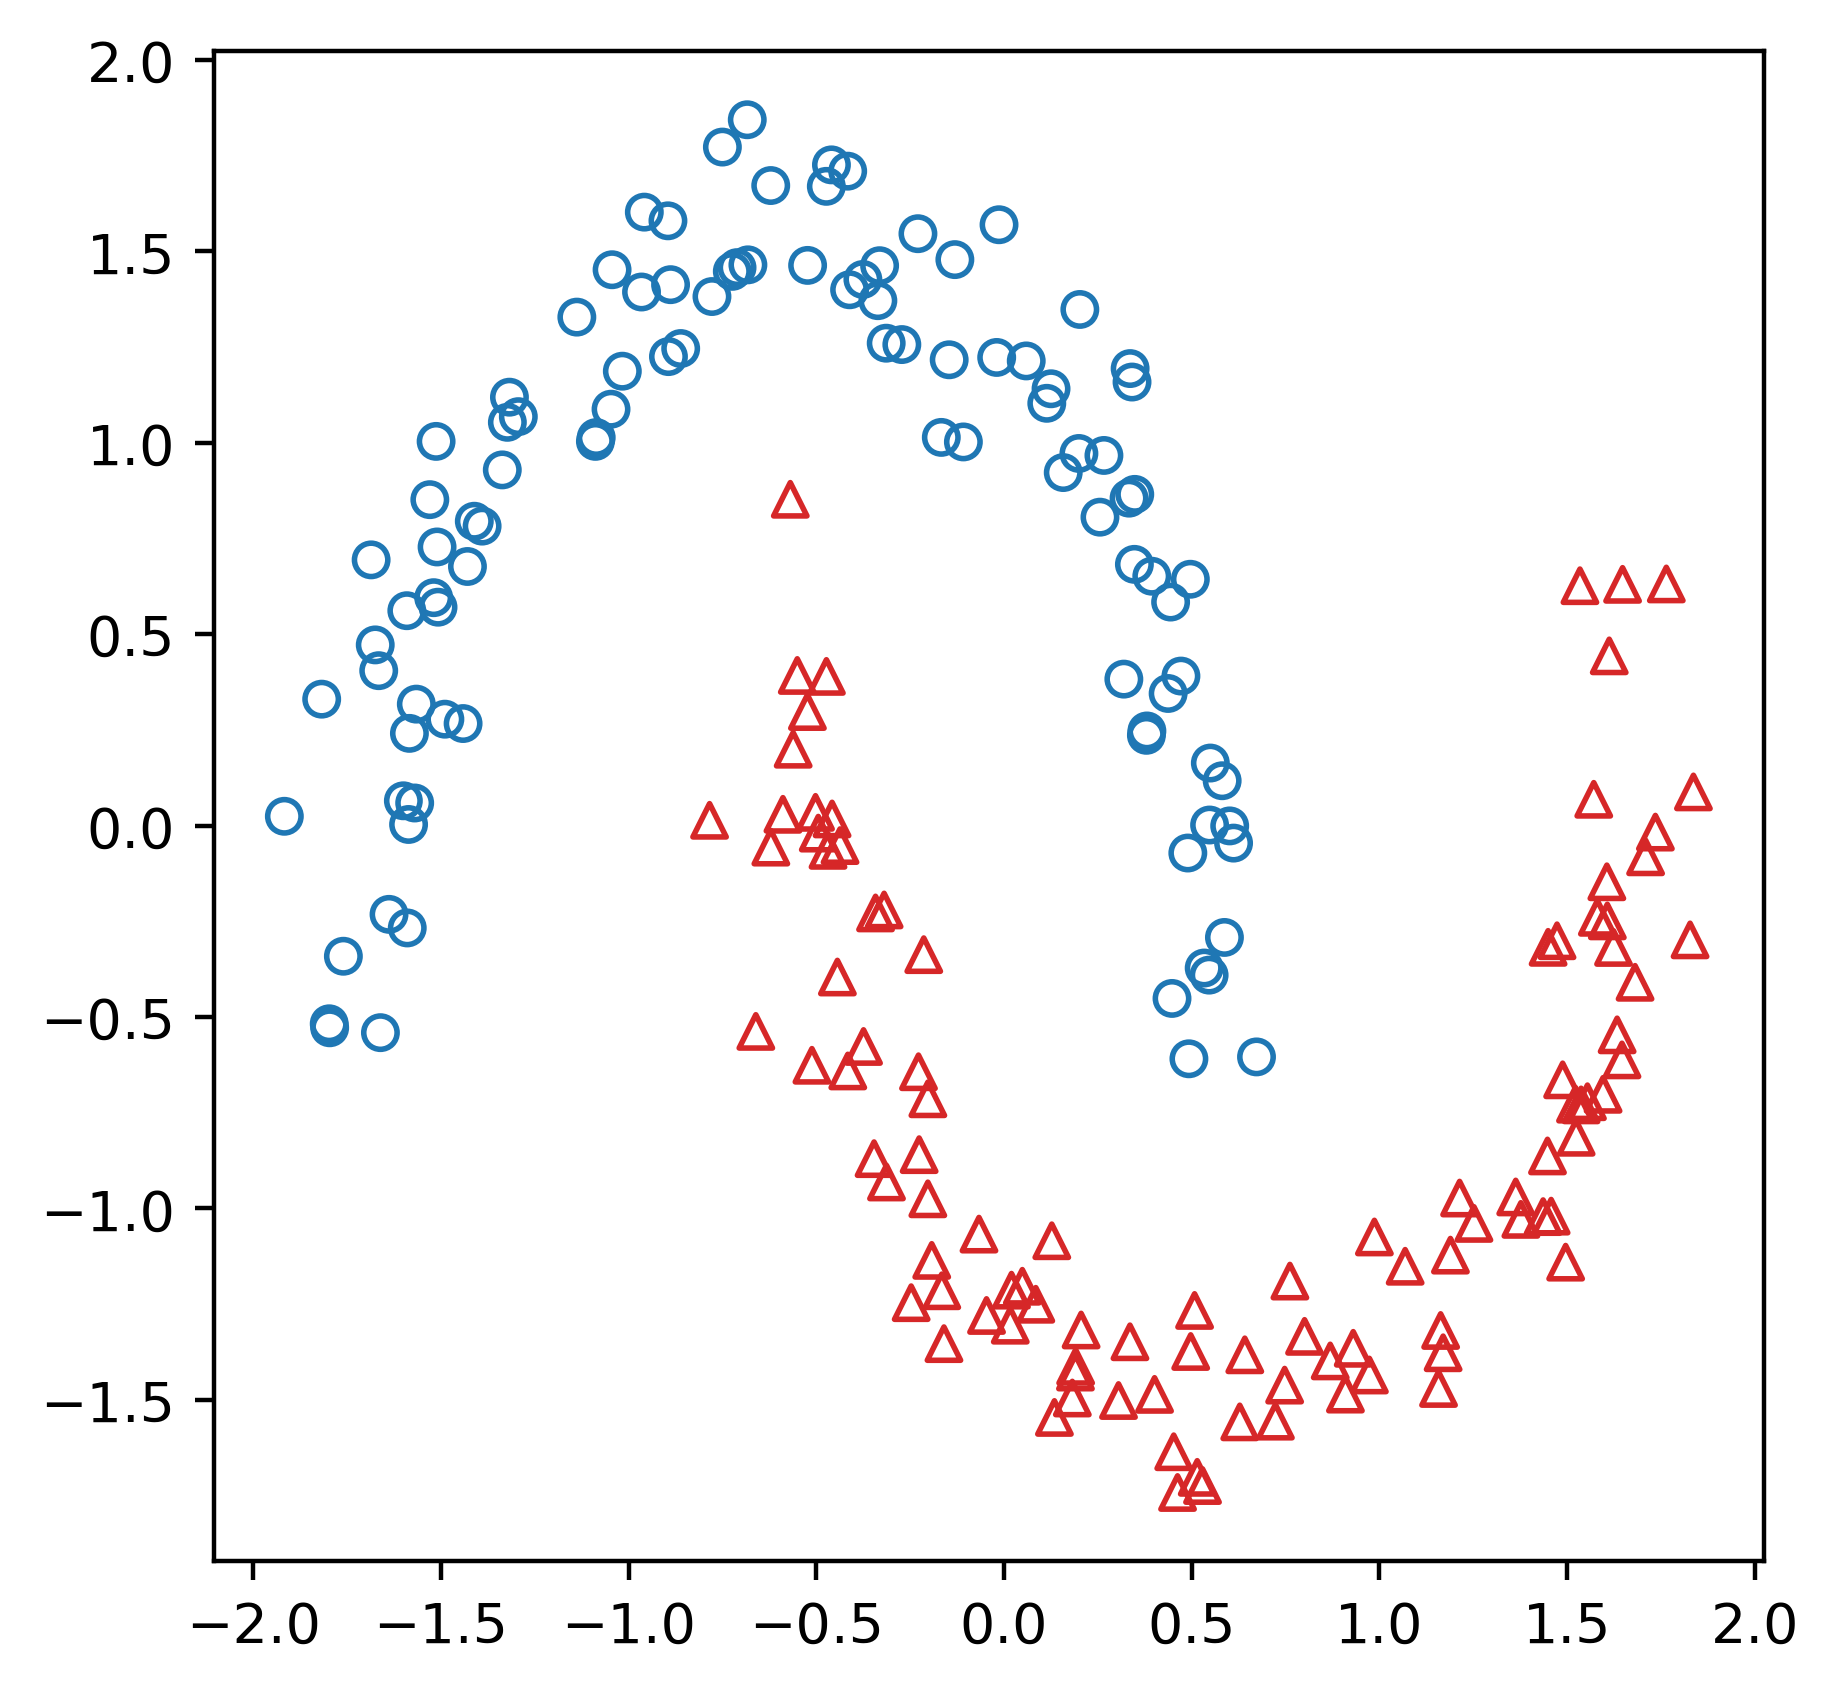
\includegraphics[width=\linewidth]{figures/data.png}  
            \caption{Two-moon dataset}
            \label{fig:data}
        \end{subfigure}
        \begin{subfigure}{.33\textwidth}
            \centering
            % include first image
            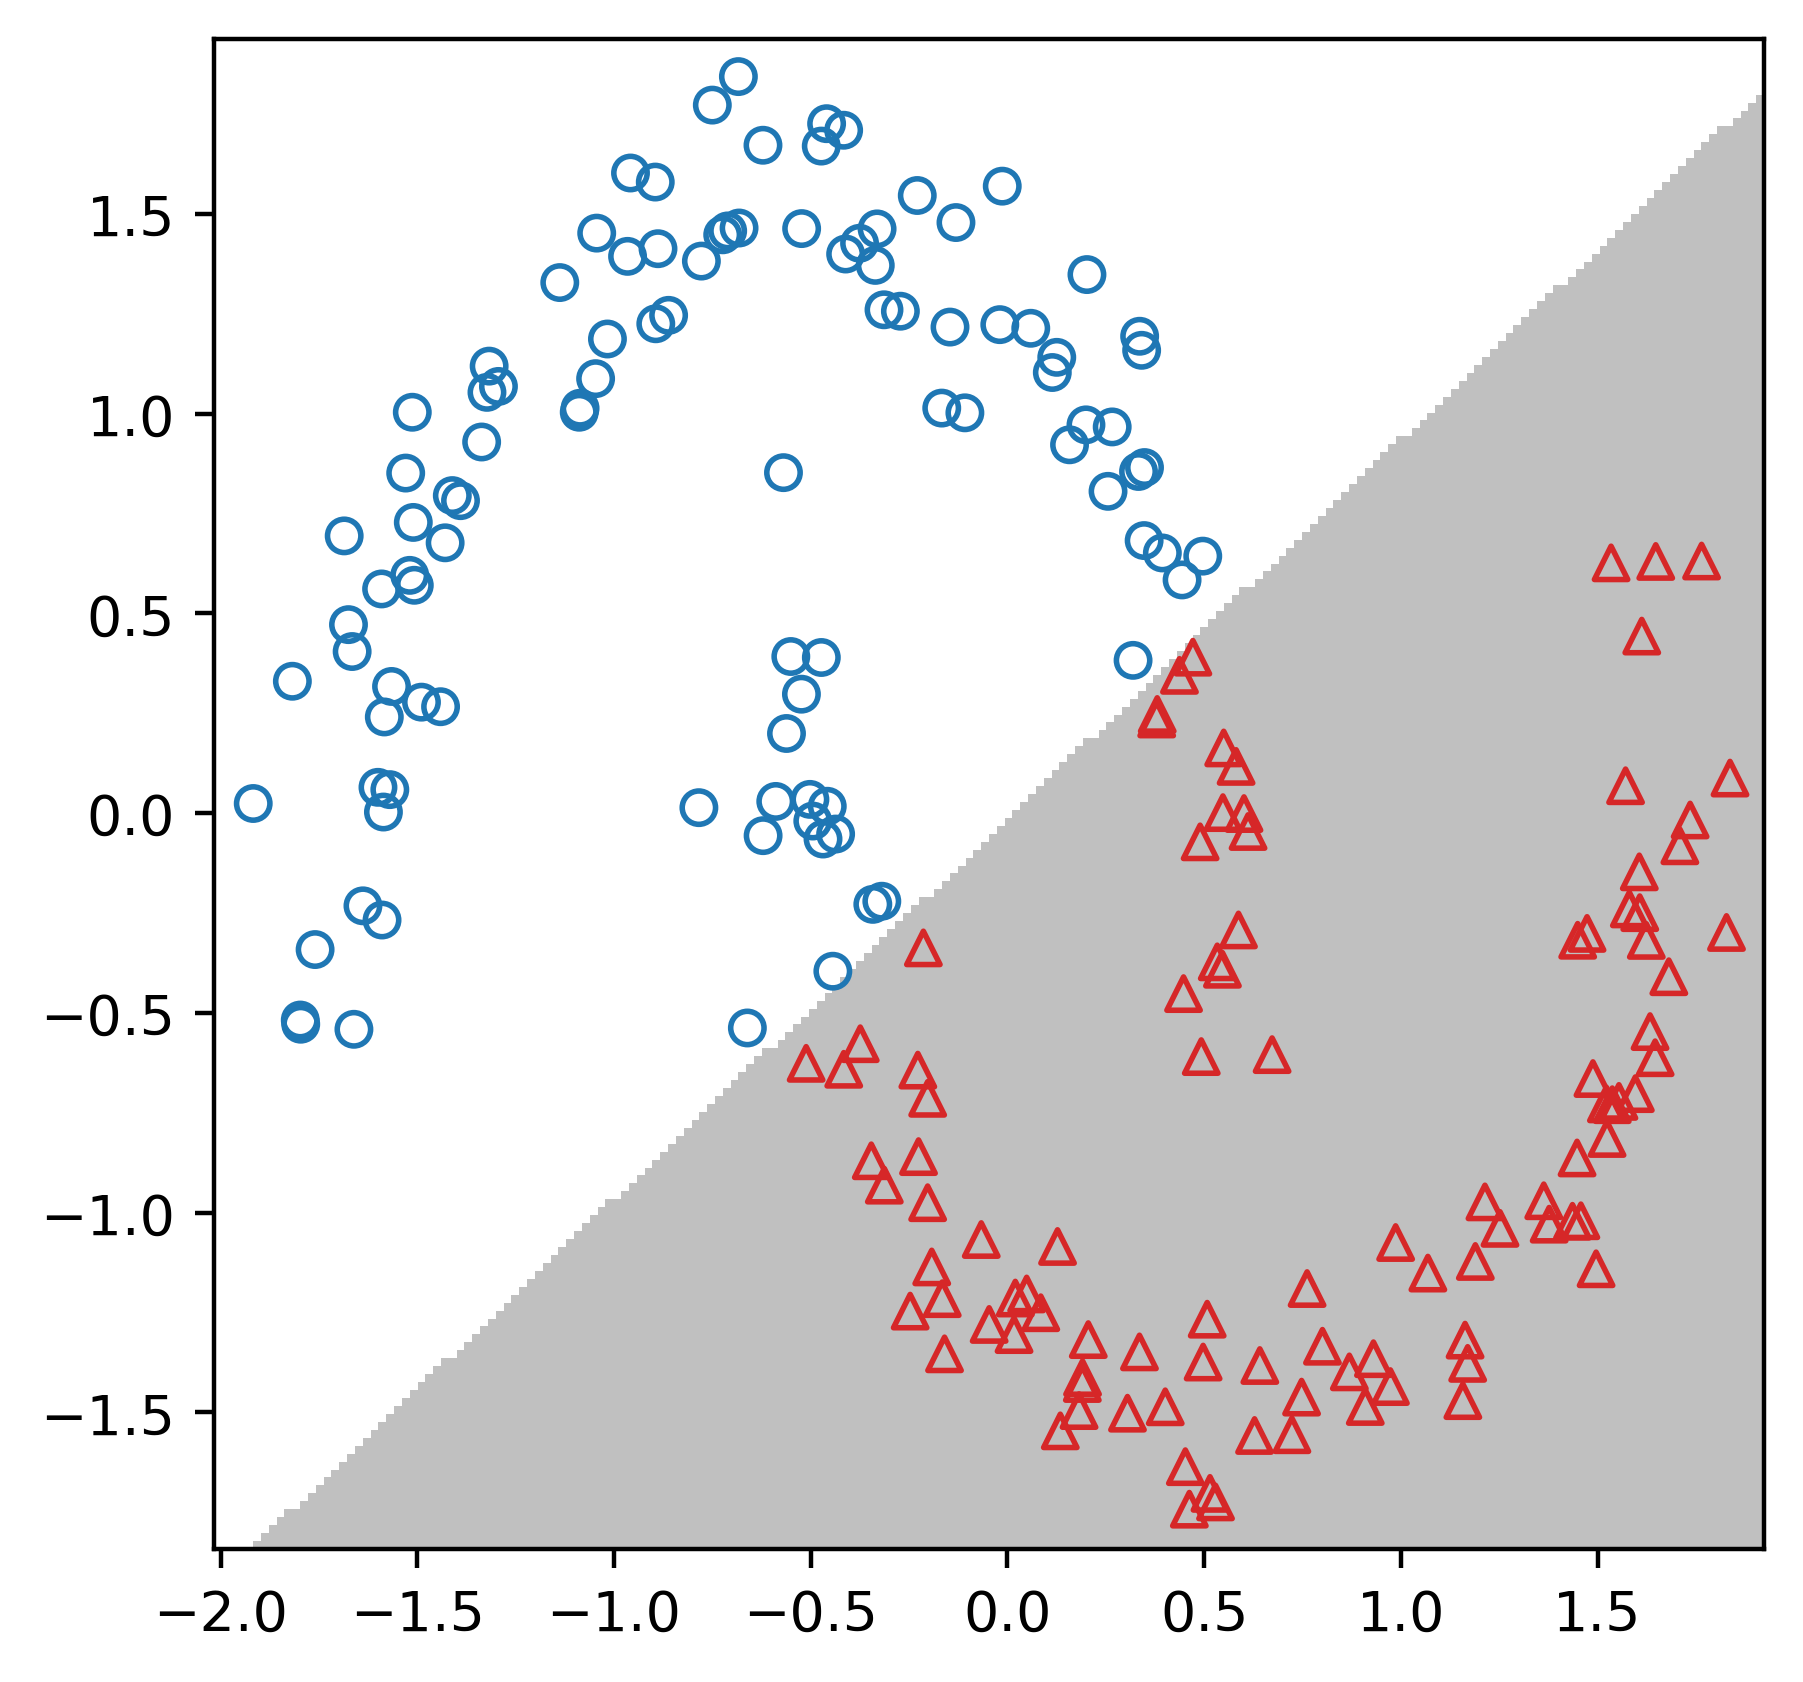
\includegraphics[width=0.98\linewidth]{figures/kmeans.png}  
            \caption{k-means}
            \label{fig:kmeans}
        \end{subfigure}
        \begin{subfigure}{.33\textwidth}
            \centering
            % include first image
            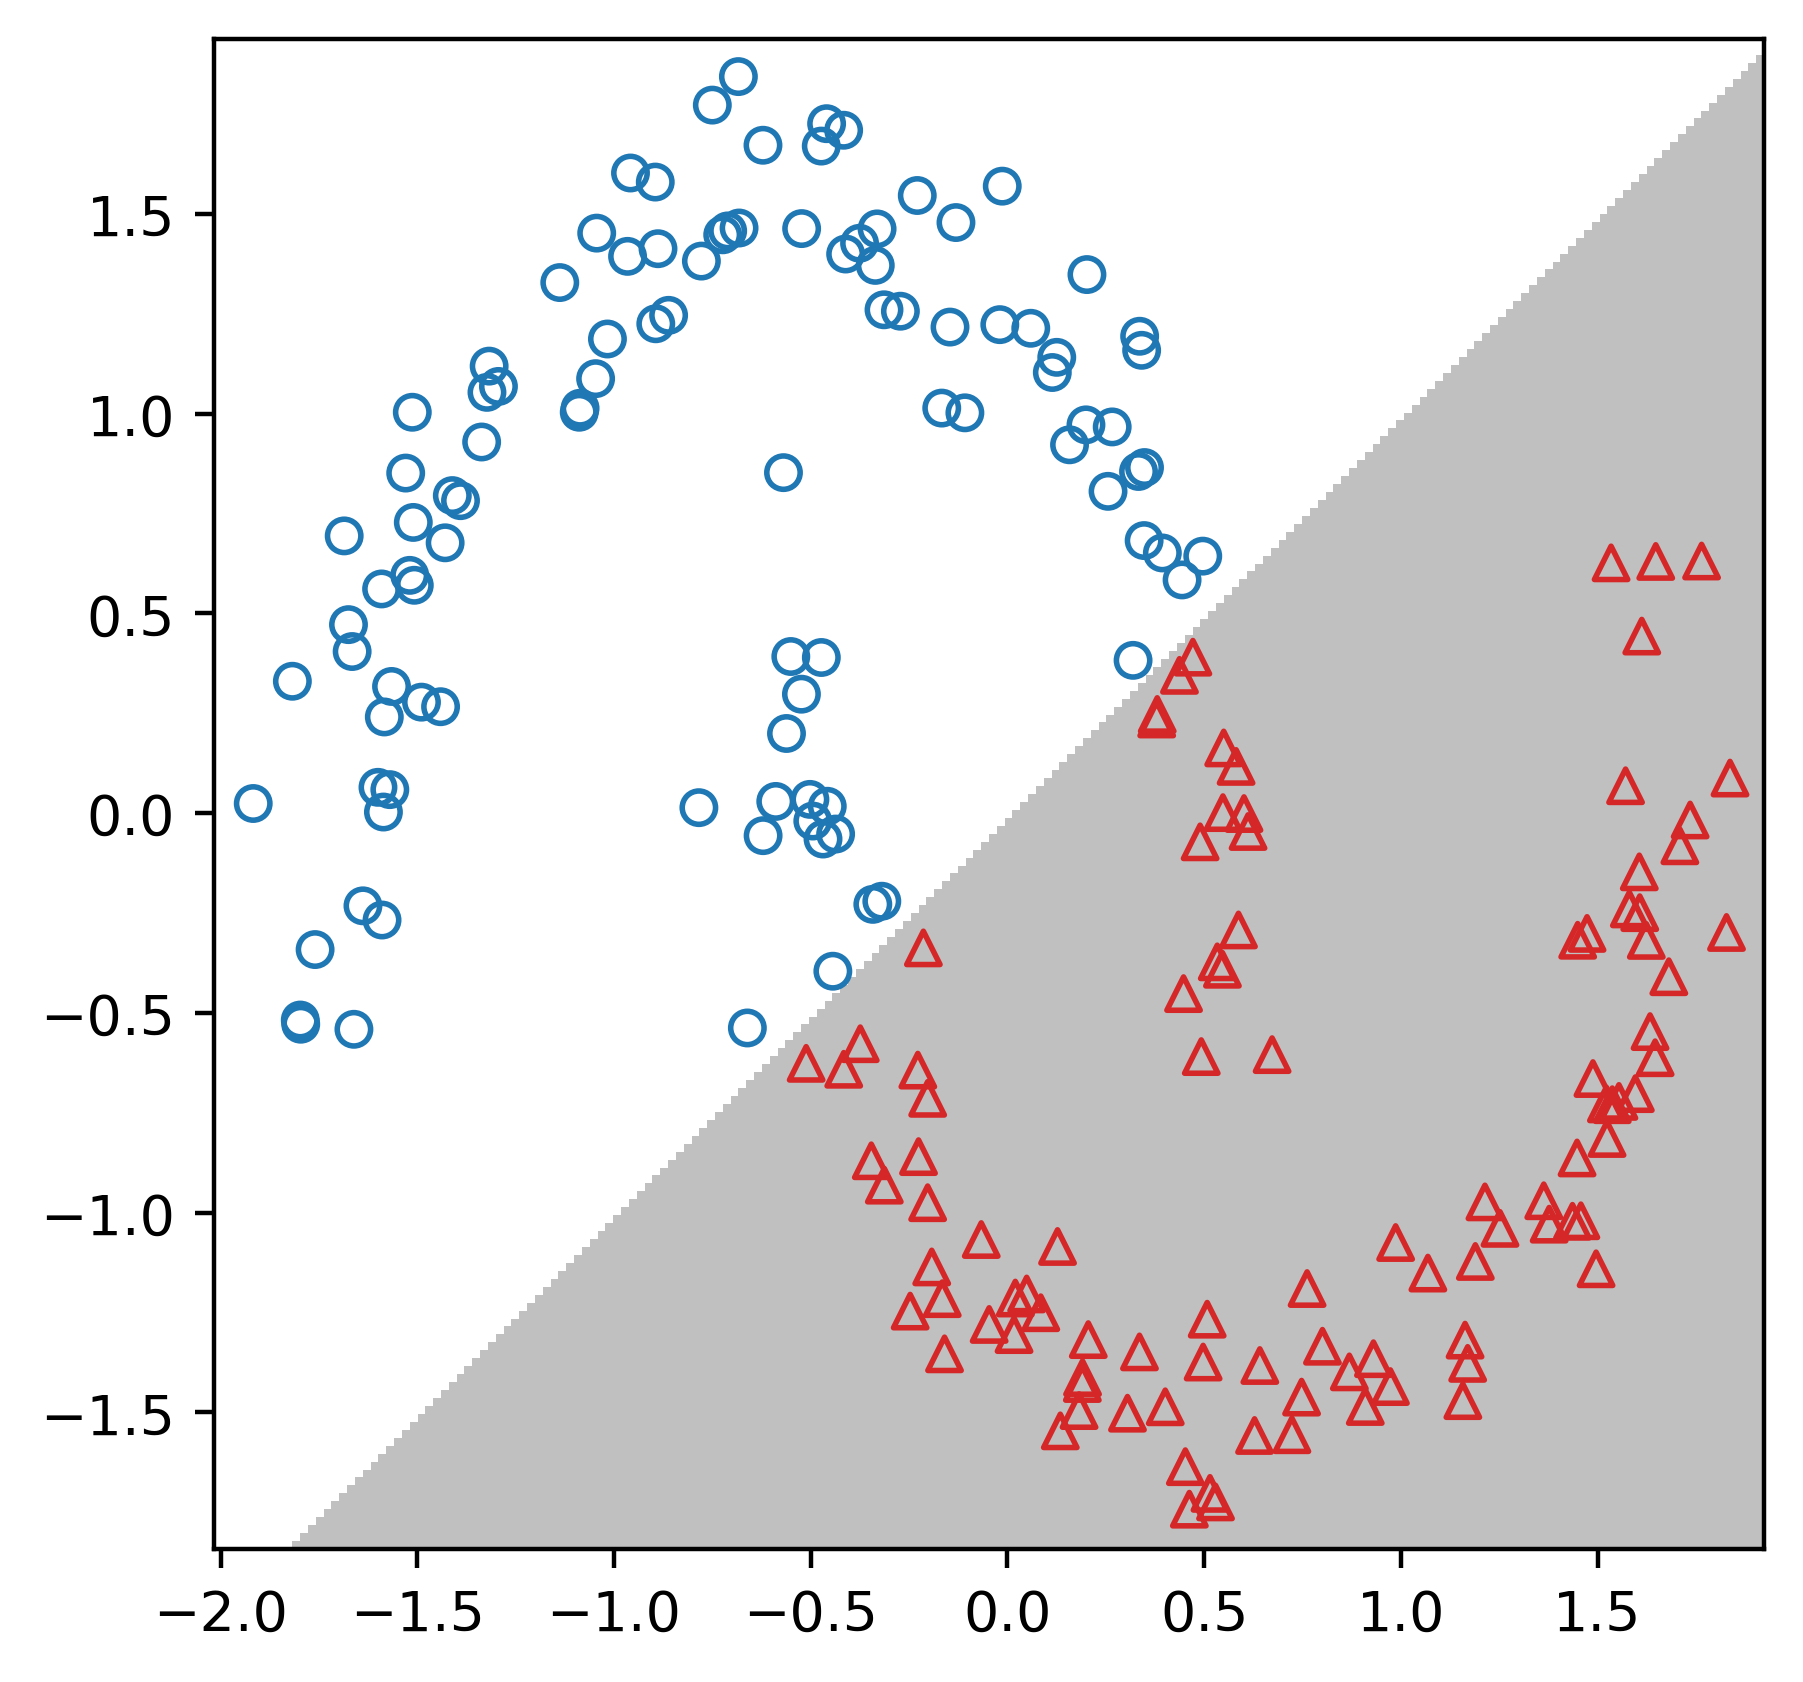
\includegraphics[width=0.98\linewidth]{figures/pca-kmeans.png}  
            \caption{PCA+k-means}
            \label{fig:pcakmeans}
        \end{subfigure}
        \newline
        
        \begin{subfigure}{.33\textwidth}
            \centering
            % include first image
            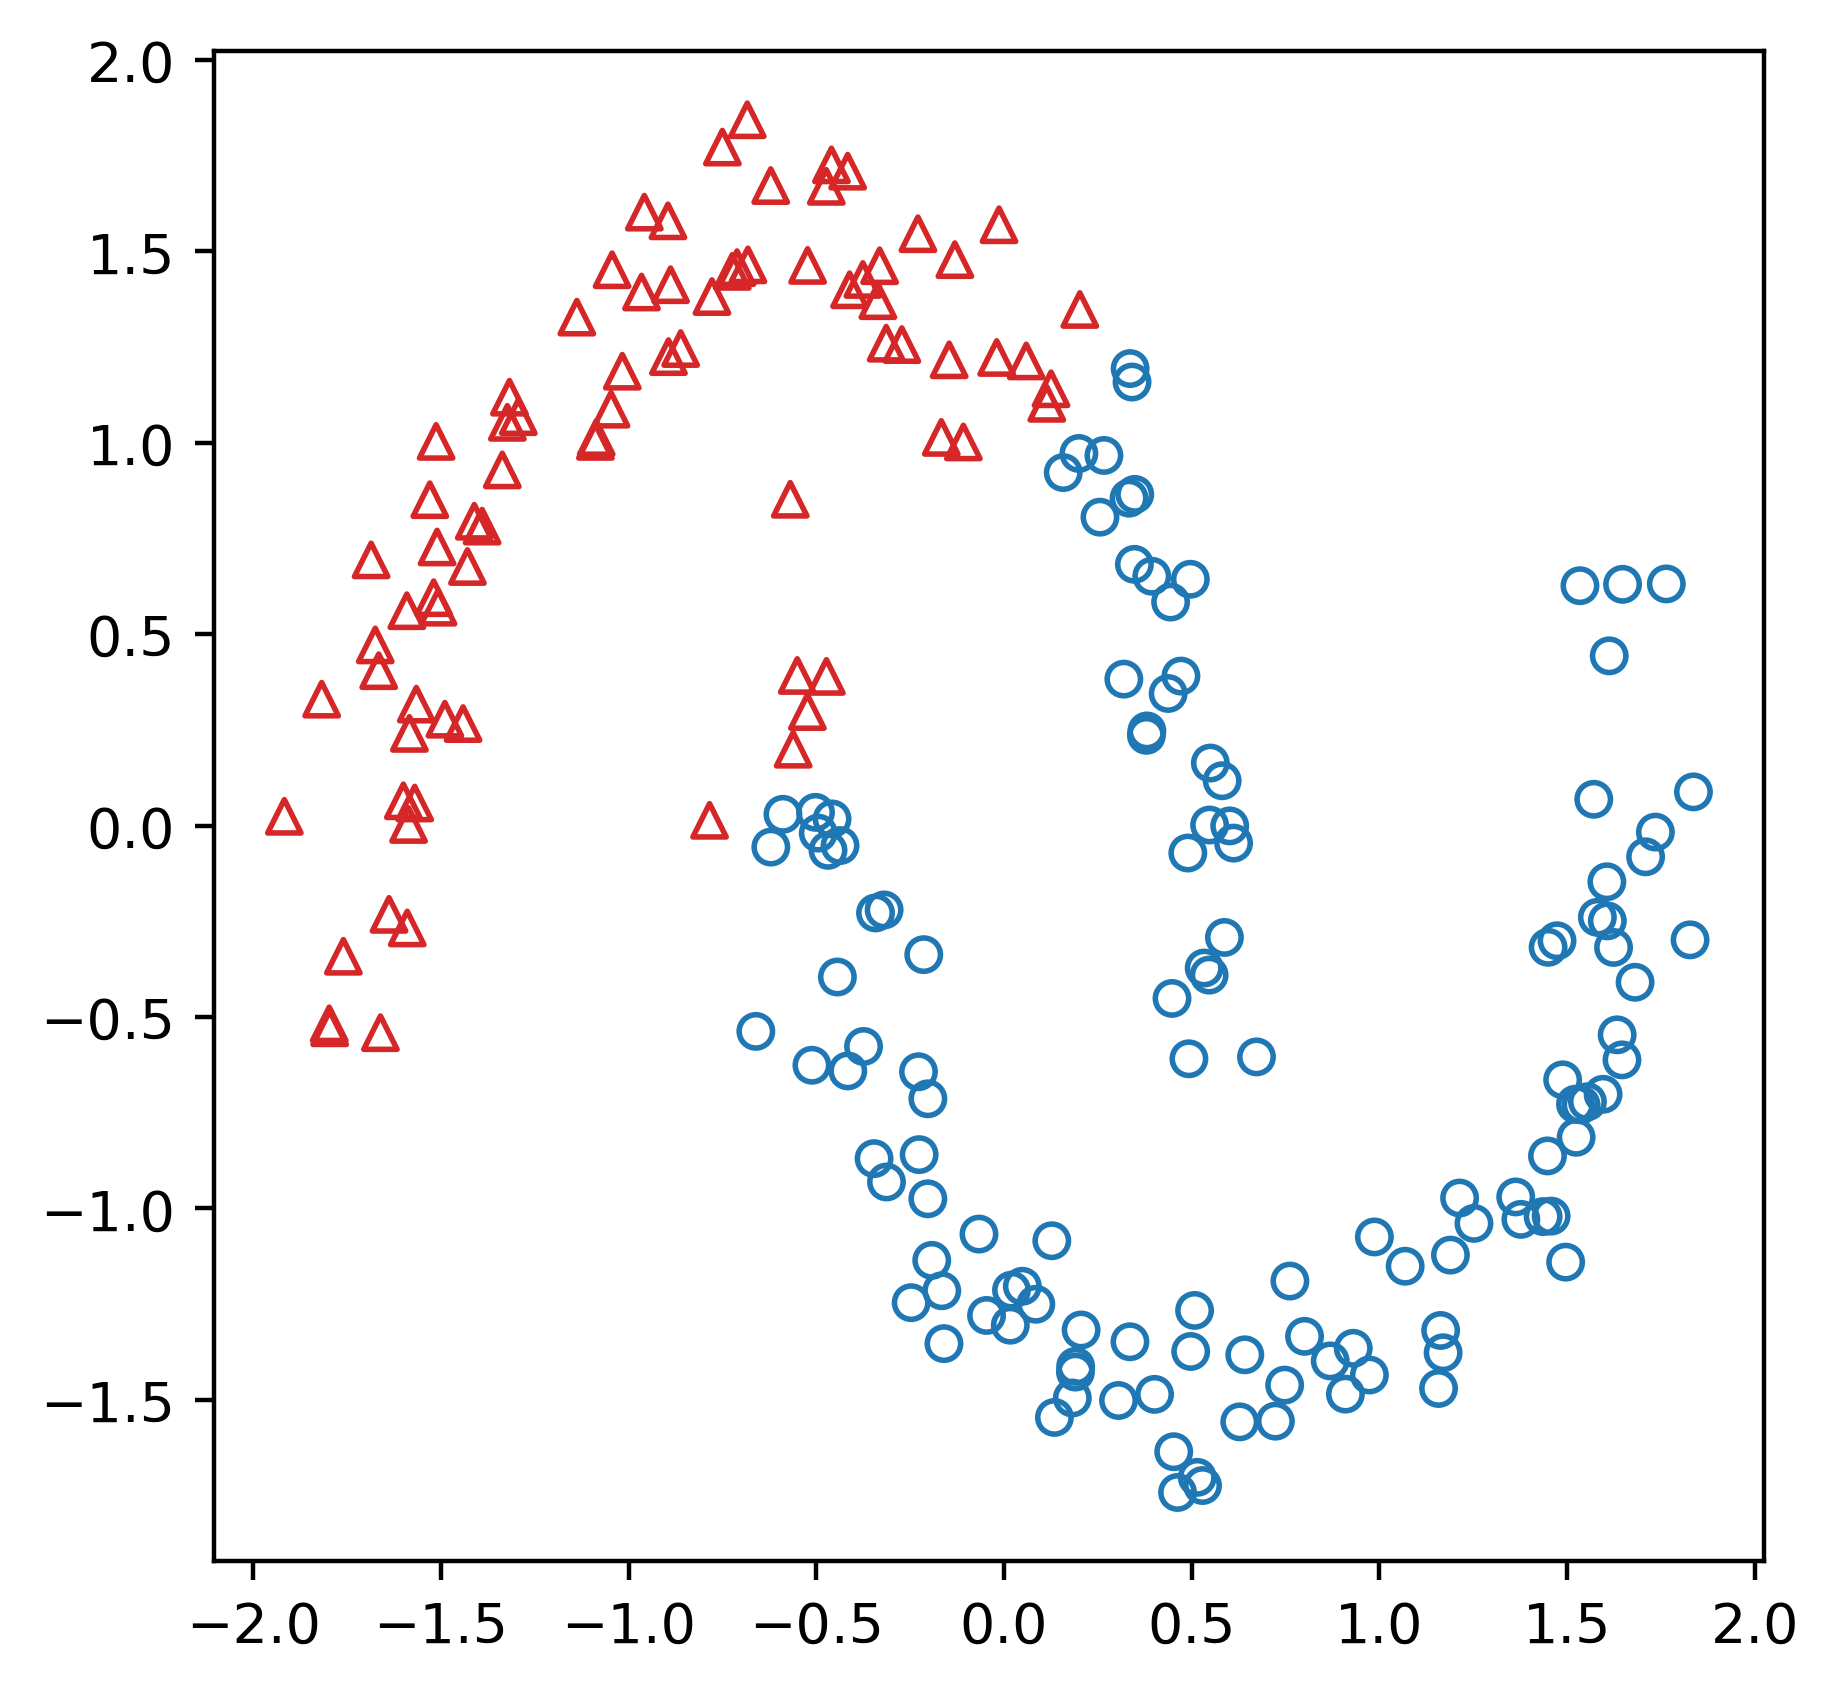
\includegraphics[width=\linewidth]{figures/nmf.png}  
            \caption{NMF}
            \label{fig:nmf}
        \end{subfigure}
        \begin{subfigure}{.33\textwidth}
            \centering
            % include first image
            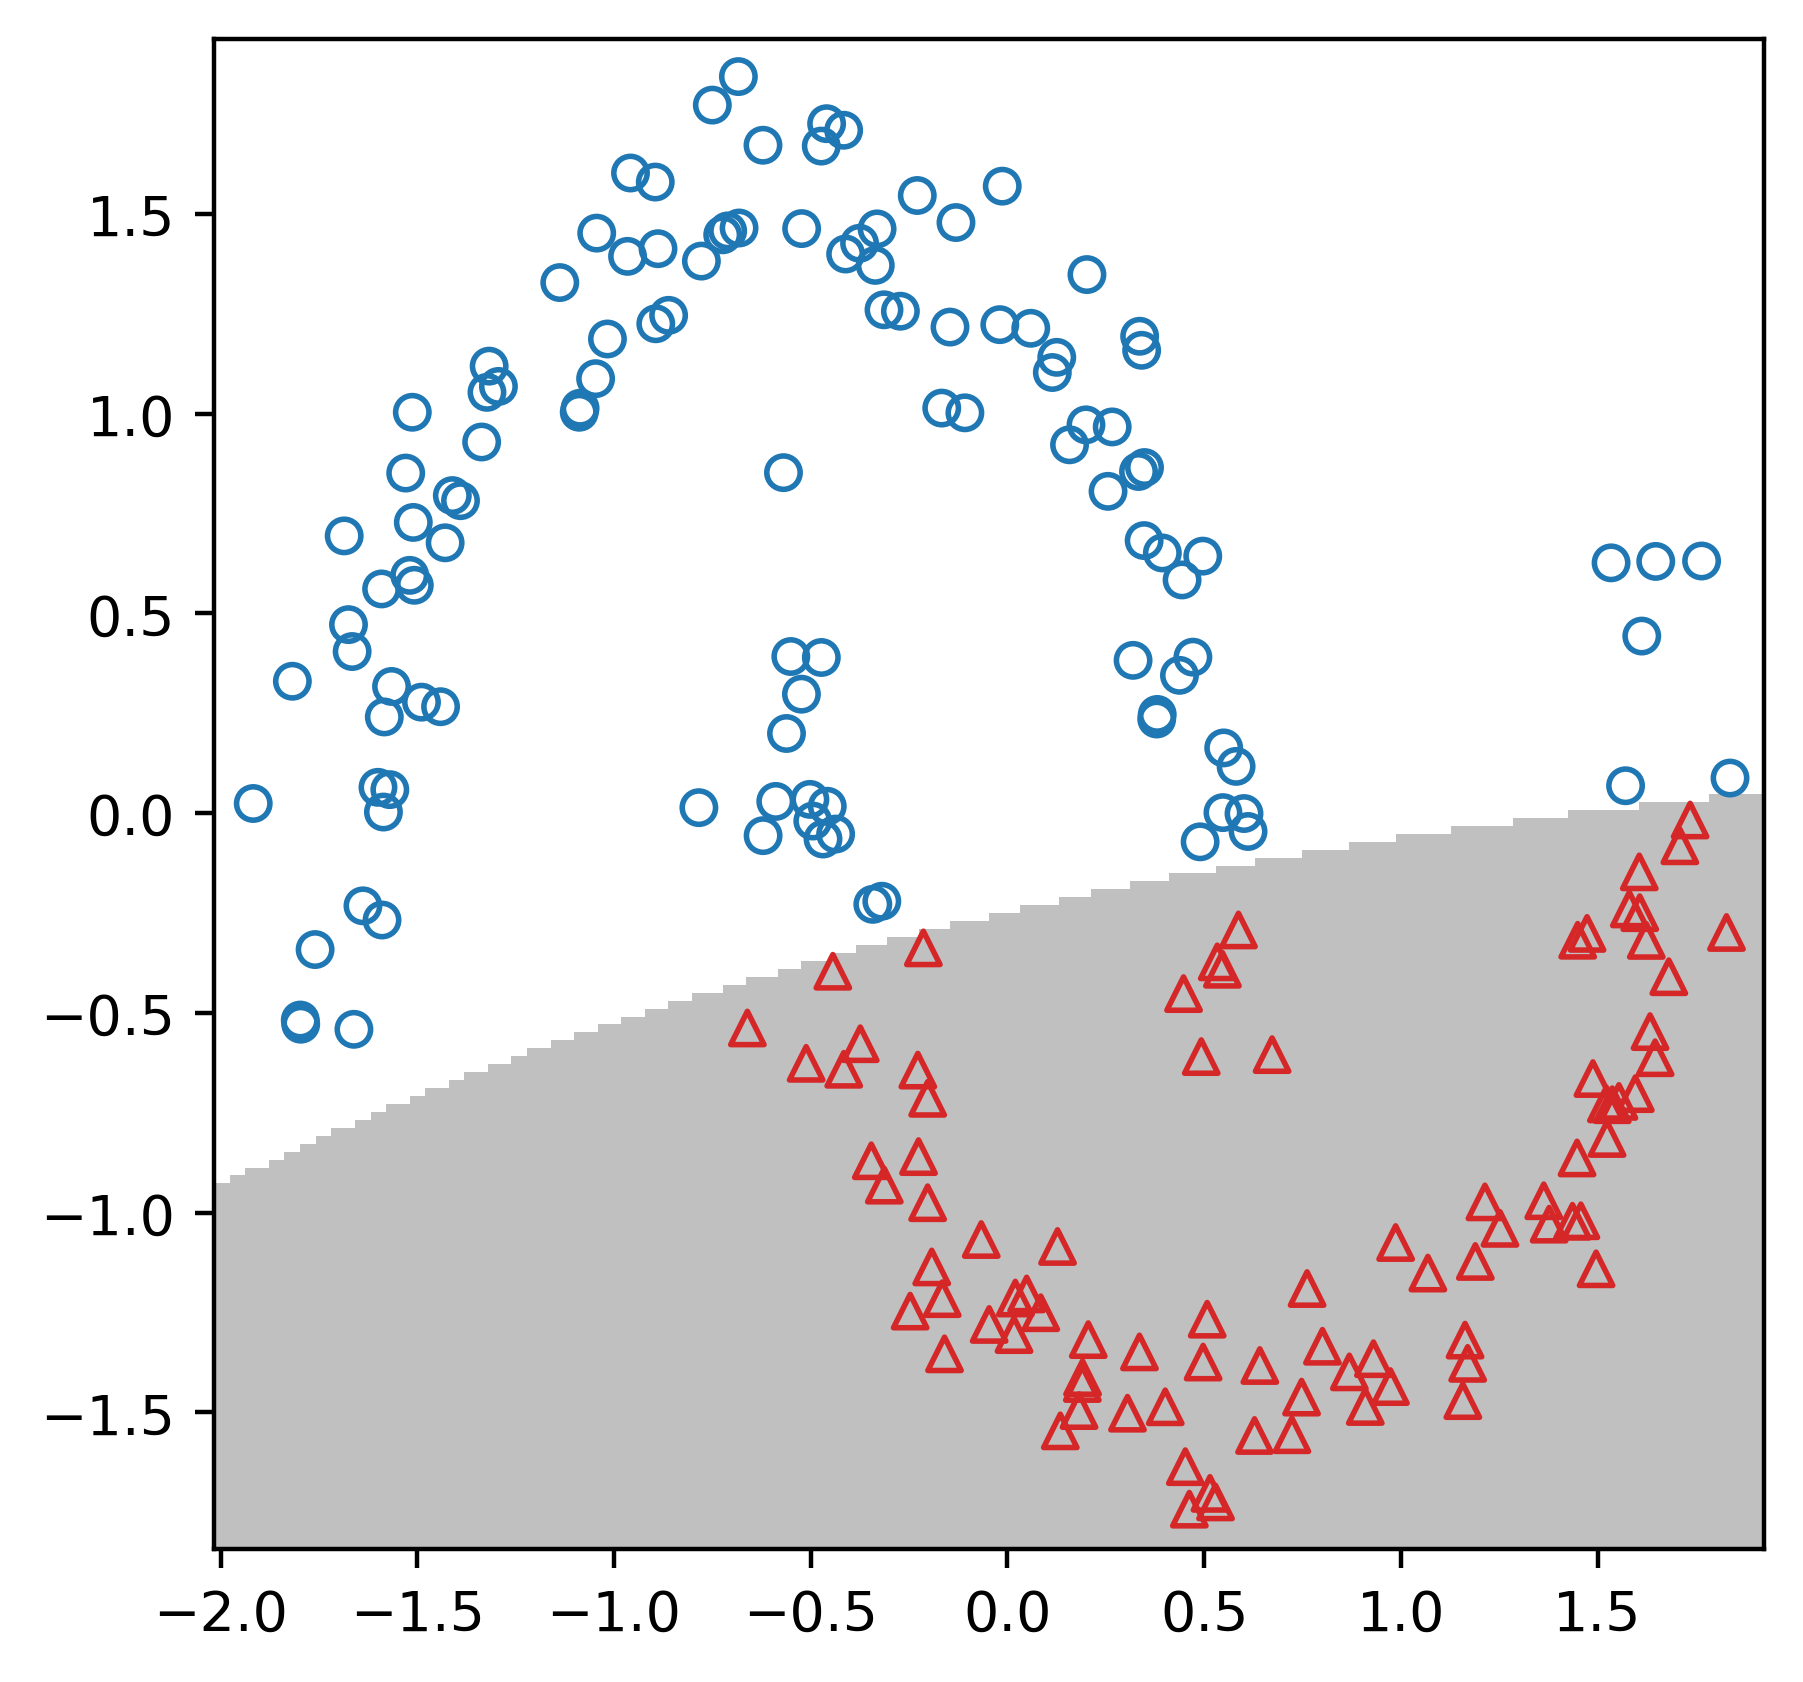
\includegraphics[width=0.98\linewidth]{figures/gmm.png}  
            \caption{GMM}
            \label{fig:gmm}
        \end{subfigure}
        \begin{subfigure}{.33\textwidth}
            \centering
            % include first image
            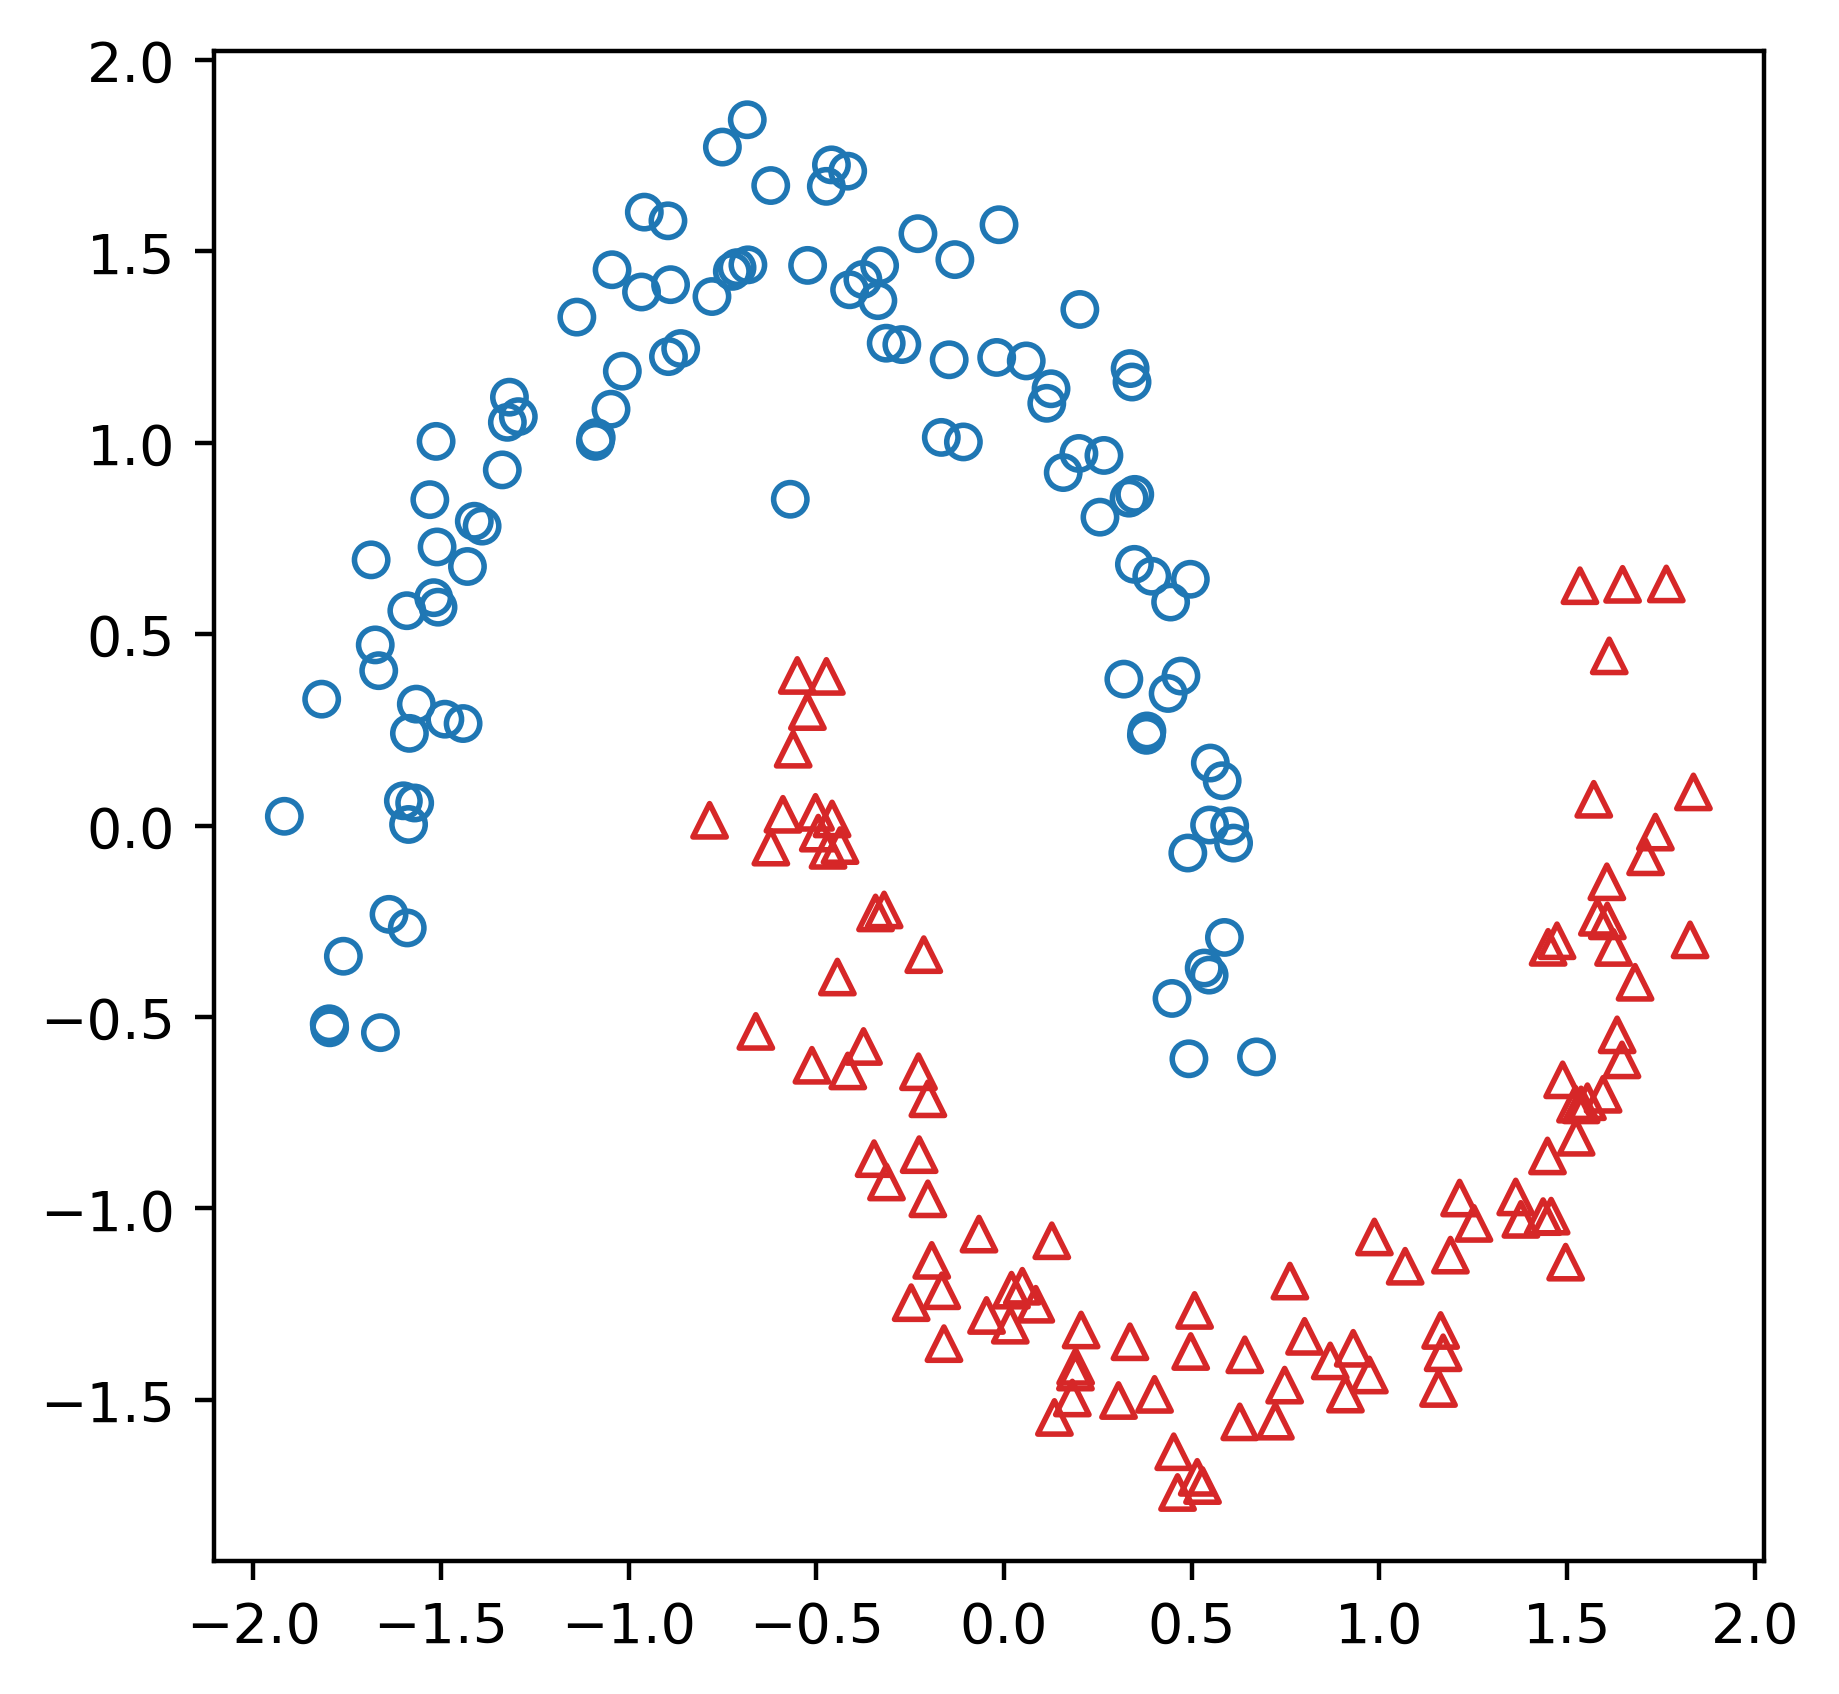
\includegraphics[width=0.98\linewidth]{figures/LapGMM.png}  
            \caption{LapGMM}
            \label{fig:lapgmm}
        \end{subfigure}
        \caption{Clustering on the two moons pattern. (a) Original data set; (b) Clustering results given by k-means with decision boundary; (c) Clustering results given by PCA and k-means with decision boundary; (d) Clustering results given by NMF; (e) Clustering results given by GMM (random initialization) with decision boundary; (f) Clustering results given by LapGMM}
    \end{figure*}

    Algorithm \ref{algo:lapgmm} shows our implementation of the LapGMM method. We made some additional assumptions that the original paper didn't mention. First, we use the same initial $\gamma=0.9$ every time we move from the E-step to the M-step. Otherwise $\gamma$ will decrease to 0 exponentially, making the smoothing process hard to converge in the late stages of the EM iteration. Second, we choose to setup a maximum iteration number for all the while loops. Unfortunately, there's no mathematical proof that decreasing $\gamma$ will result in a larger $\mathcal{L}(\Theta)$ so we introduce an early stopping mechanism to avoid endless loops.

\section{Experiment}\label{sec:experiment}

    \subsection{Experiment Setup}
    
    \subsubsection{Implementation of GMM}
    
    The initial values of the GMM are generated using uniform distribution sampling, random sampling, and k-means. In uniform distribution sampling, mean and variance vectors are obtained from $K$ equally sized clusters after shuffling the observations. The prior probability of each cluster is identical because of the same observations' membership to each cluster. In random sampling, the mean vector is generated by $K$ randomly selected observations. Each observation is assigned to the nearest cluster with one mean value as the center. The prior probability and variance are calculated cluster by cluster based on the sample variance and the number of elements. In the k-means setting, k-means with given number of clusters is conducted before the calculation of three parameter vectors based on the elements in each cluster.  
    %Based on the number of clusters given, Gaussian distributions are randomly generated with means selected from a uniform distribution across the upper and lower bounds of the observations and variances selected from a uniform distribution ranging from zero to twice the variance of the observations. The vector of probabilities associated with the frequency of the observations' membership to each cluster is chosen such that all elements are equal and sum to one.
    
    After initialization, EM process is performed in estimation of the parameters. The process iterates until either the log-likelihood or the number of iterations reaches the maximum. Note that BIC is used in selection of the optimal number of clusters.
    %the squared sum of each element in the difference between the matrix of probabilities of each data point's membership to each cluster and its previous update is below a given threshold or the given maximum number of iterations is reached.
    
        \subsubsection{Fitting GMM on S\&P 500 Index Data}
    
    S\&P 500 index data was downloaded from Yahoo Finance. We used adjusted price from 2000-01-01 to 2021-03-14. Weekly return was calculated as log return.
    
    For the GMM model, we used different initialization methods and number of components to ensure the robustness of the result. Initialization methods included uniform distribution initialization, random initialization and K-means initialization. The parameters of the algorithm were listed below. The optimal number of clusters was chosen using BIC and the value is 3.
    
    \begin{table}[H]
        \centering
        \begin{tabular}{|l|l|l|}
            \hline
            Symbol & Description & Value  \\
            \hline
            $(m.d)$ & Size of the dataset & $1105\times 1$\\ 
            \hline
            $K$ & Number of clusters & $1 \sim 15$\\
            \hline
            $\delta_{\mathrm{EM}}$ & termination value of EM iteration & $10^{-2}$\\
            \hline
            $N_{\mathrm{EM}}$ & max iteration of EM & $100$\\
            \hline
        \end{tabular}
        \caption{Parameters of GMM Algorithm}
        \label{tab:parameter-gmm}
    \end{table}
    
    \subsubsection{Implementation of LapGMM}
    
    We implemented LapGMM based on Algorithm \ref{algo:lapgmm} with the following parameters
    
    \begin{table}[H]
        \centering
        \begin{tabular}{|l|l|l|}
            \hline
            Symbol & Description & Value  \\
            \hline
            $(m.d)$ & Size of the dataset & $200\times 2$\\ 
            \hline
            $K$ & Number of clusters & $2$\\
            \hline
            $p$ & Number of nearest neighbors & $5$\\
            \hline
            $\lambda$ & Regularization parameter & $100$\\
            \hline
            $\delta_{\mathrm{EM}}$ & termination value of EM iteration & $10^{-6}$\\
            \hline
            $\delta_{\mathrm{NR}}$ & termination value of Newton method & $10^{-6}$\\
            \hline
            $N_{\mathrm{EM}}$ & max iteration of EM & $50$\\
            \hline
            $N_{\mathrm{NR}}$ & max iteration of Newton method & $2000$\\
            \hline
            $N_{\mathrm{M}}$ & max iteration of M-step & $500$\\
            \hline
        \end{tabular}
        \caption{Parameters of LapGMM Algorithm}
        \label{tab:parameter-lapgmm}
    \end{table}
    


    \subsection{Results and Analysis}
    
    
    
    
    
    \subsubsection{K-means and GMM for Two Moons Example}
    
    For the two moons example shown in Figure \ref{fig:data}, we can see in Figure \ref{fig:kmeans} to \ref{fig:gmm} that k-means, NMF and Gaussian Mixture Model (GMM) fail to identify the moon clusters. The linear decision boundary of k-means and quadratic decision boundary of GMM limited the clustering ability in two-moon dataset. Although NMF doesn't have a clear decision boundary, it models each cluster as a linear combination of the data points. So it's difficult to cluster the ambient space.
    
    Both k-means and GMM identify clusters based on “round” data in space; one using Voronoi cells and the other using “ellipses”. Although GMM makes some assumptions on the underlying distribution of input data, in the two moons example it still fails to consider the submanifolds on which the underlying moon distributions are sampled from. It is clear from a quick examination of figure \ref{fig:data} that the two moons example has an intrinsic “submanifold” of the ambient space. Neither k-means nor GMM incorporates this geometric structure, giving us an answer to \textbf{RQ1} and \textbf{RQ2}. In order to come up with a method that could work for the two moons example, the underlying geometry of the probability distributions needs to be considered.
    
        
    \subsubsection{GMM for S\&P 500 index density estimation}
    
    GMM can be used not only as a clustering algorithm but also as a density estimation algorithm. Examining the density of weekly returns of the S\&P 500 index, it has a heavier tail than normal distribution. The fat tail feature of index return is also referred to as tail risk, which is attributed to the occurrence of extreme events and abnormal returns. We fit a GMM model to estimate the distribution of weekly returns of the S\&P 500 index, and investigated whether this model is able to reproduce correctly the tails of the distribution.
    
    The tail feature of the obtained distribution was examined using three different approaches. In Figure \ref{fig:log_plot_tail}, log plot shows the logarithmic scale of tail probability along the weekly return. When the weekly return is small and near the center of the distribution, the GMM distribution fits the true data much better than normal distribution. However, when the weekly return is large and at the tail of the distribution, it approaches normal distribution in an asymptotic manner. To verify GMM's failure in reproducing the tails of S\&P, we quantitatively deduced the downward trend of S\&P original data by fitting a linear model with no intercept. The $R^2$ of the fitted model is over 98$\%$, indicating the S\&P original data declines at a rate of $\exp(-at), a>0$, which is slower than the declining rate of GMM and normal distribution. Both of these methods only capture a part of the tail risk and thus fail to reproduce correctly the tails of the true data.
    %which can be asymptotically estimated by a polynomial decay function.
    
     \begin{figure}[h]
        \centering
        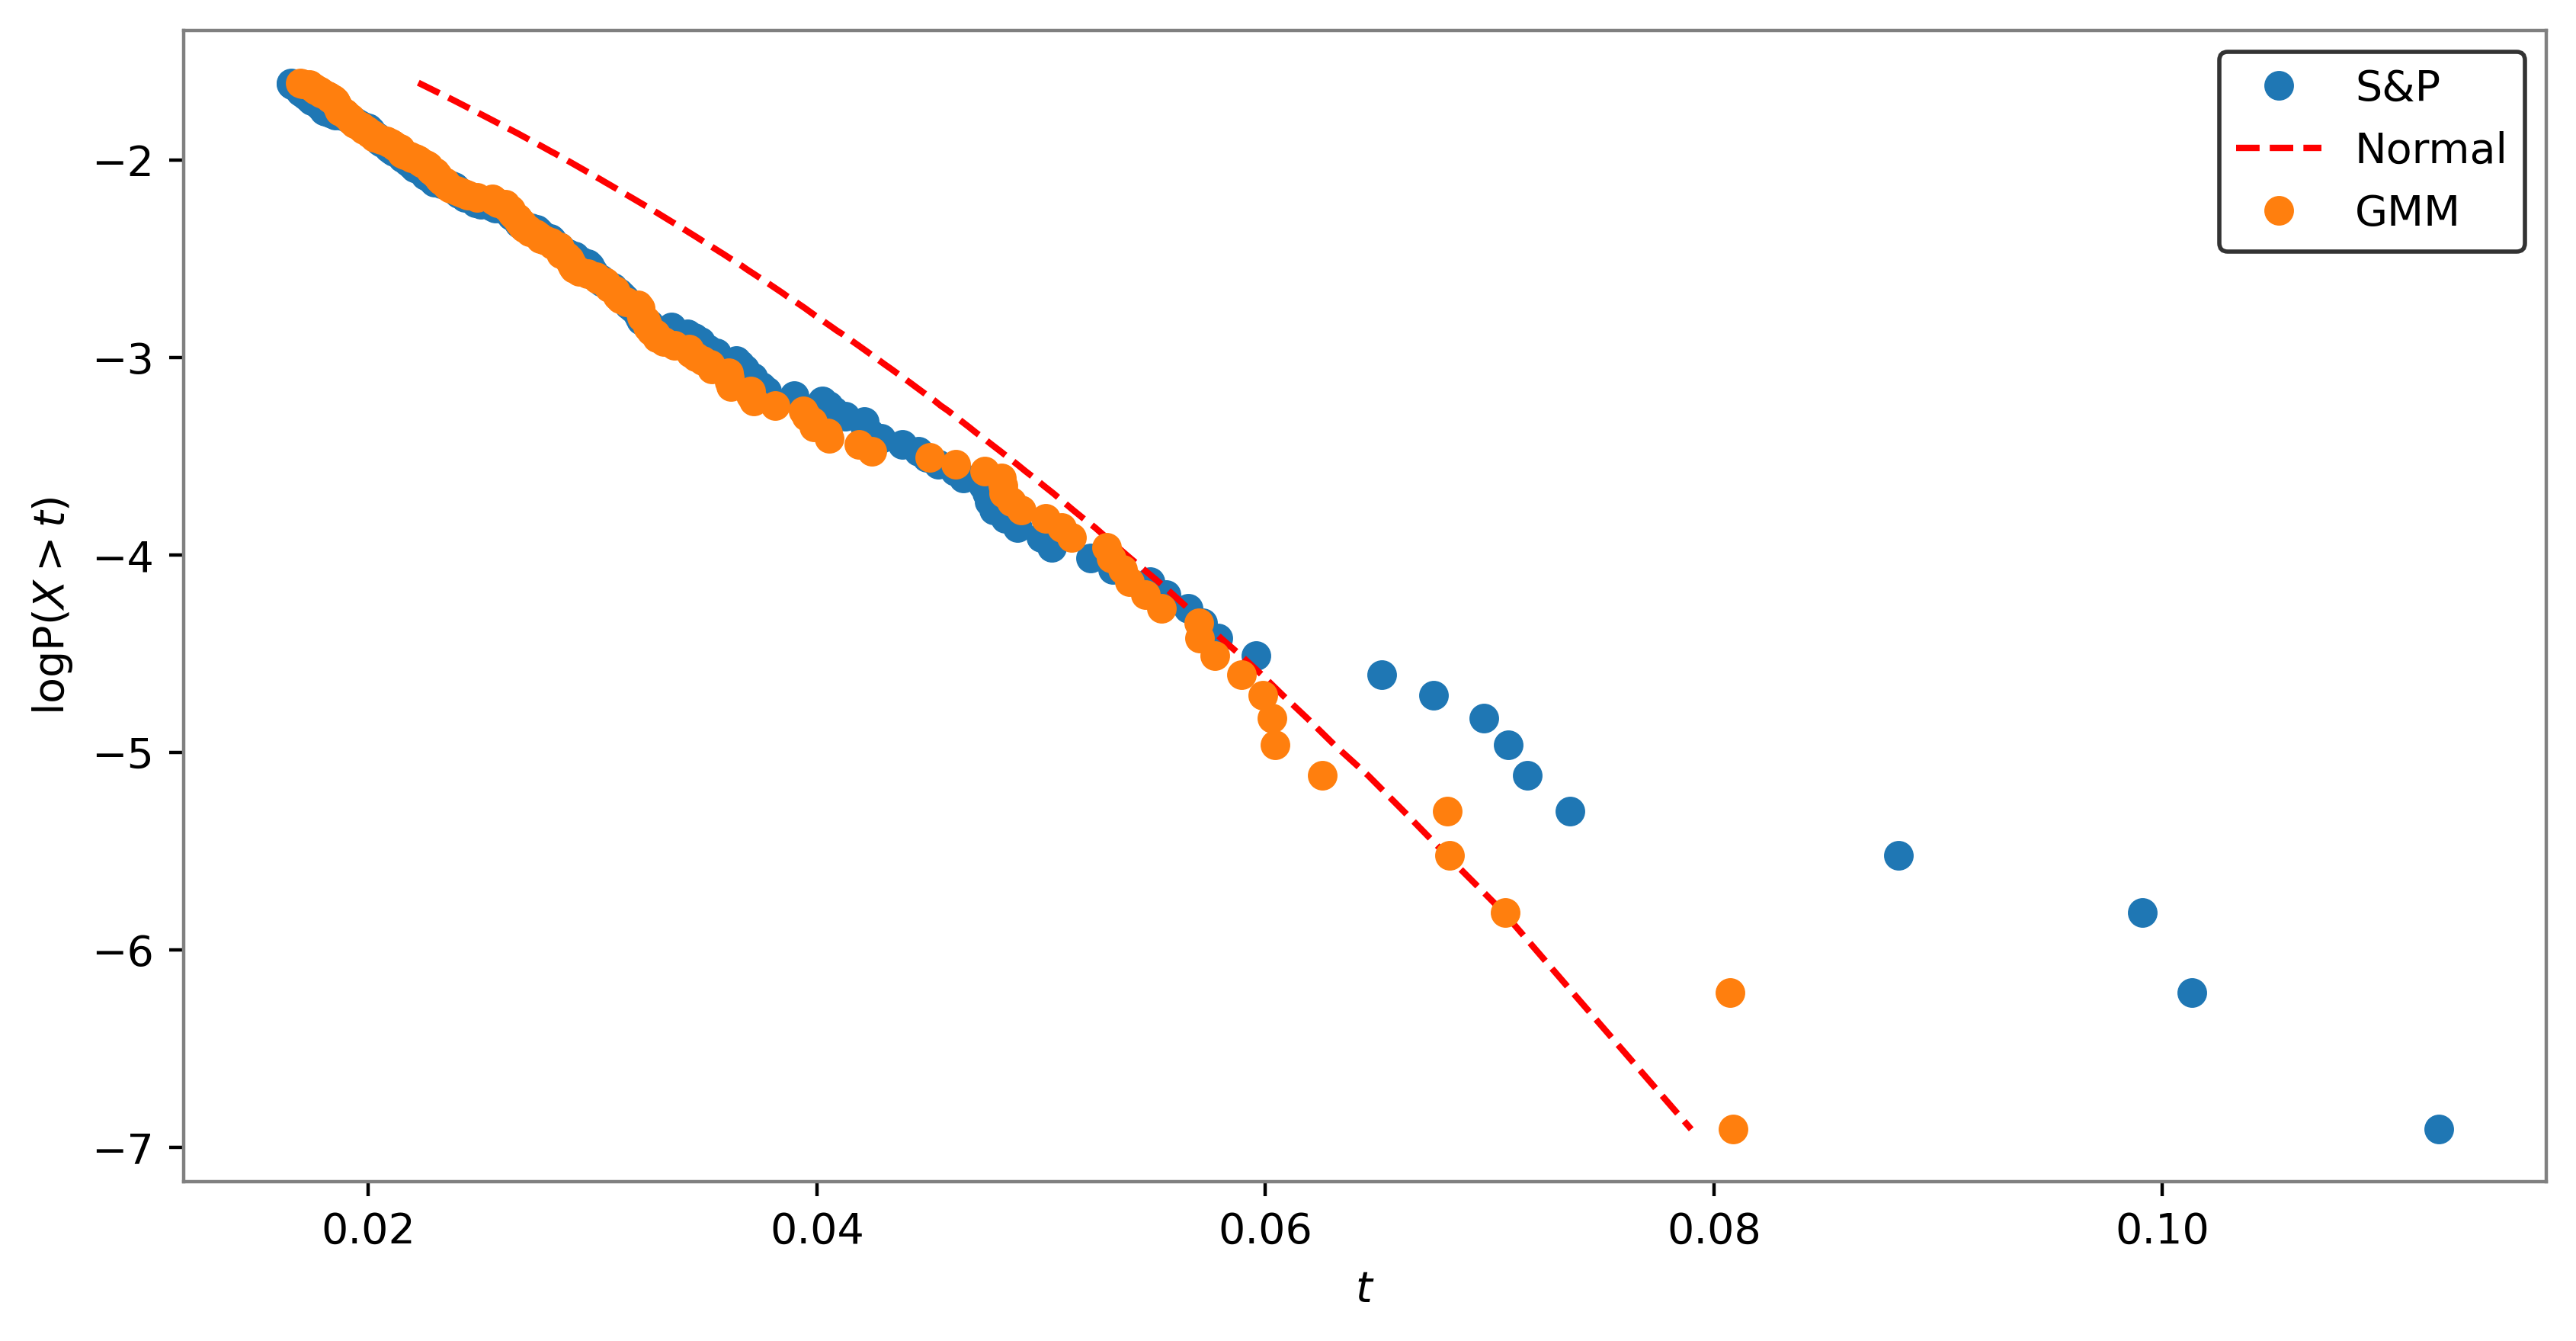
\includegraphics[width=3.5in]{figures/log_plot_tail.png}
        \caption{Log plot of the tail. When the weekly return is small and near the center of the distribution, the GMM distribution fits the true data much better than normal distribution. When the weekly return is large and at the tail of the distribution, it approaches normal distribution in an asymptotic manner.}
        \label{fig:log_plot_tail}
    \end{figure}
     
    
    Q-Q plot is another way to check the tail pattern. The Q-Q plot of S\&P 500 index return (Figure \ref{fig:qqplot_sp}) shows a downward deviation at the left and an upward deviation at the right, which conforms to the fat tail pattern (\textbf{RQ3}). As is shown in Figure \ref{fig:qqplot}, if we only used one component in the GMM model, the fitted distribution is also normal. It's trivial that they don't have fat tail as is shown in the first column. When we used more than one components, the Q-Q plots all show similar fat tail pattern no matter what initialization methods we used. The result indicates that the distribution fitted by GMM does capture at least a part of the fat tail characteristics.
    
        \begin{figure}[h]
        \centering
        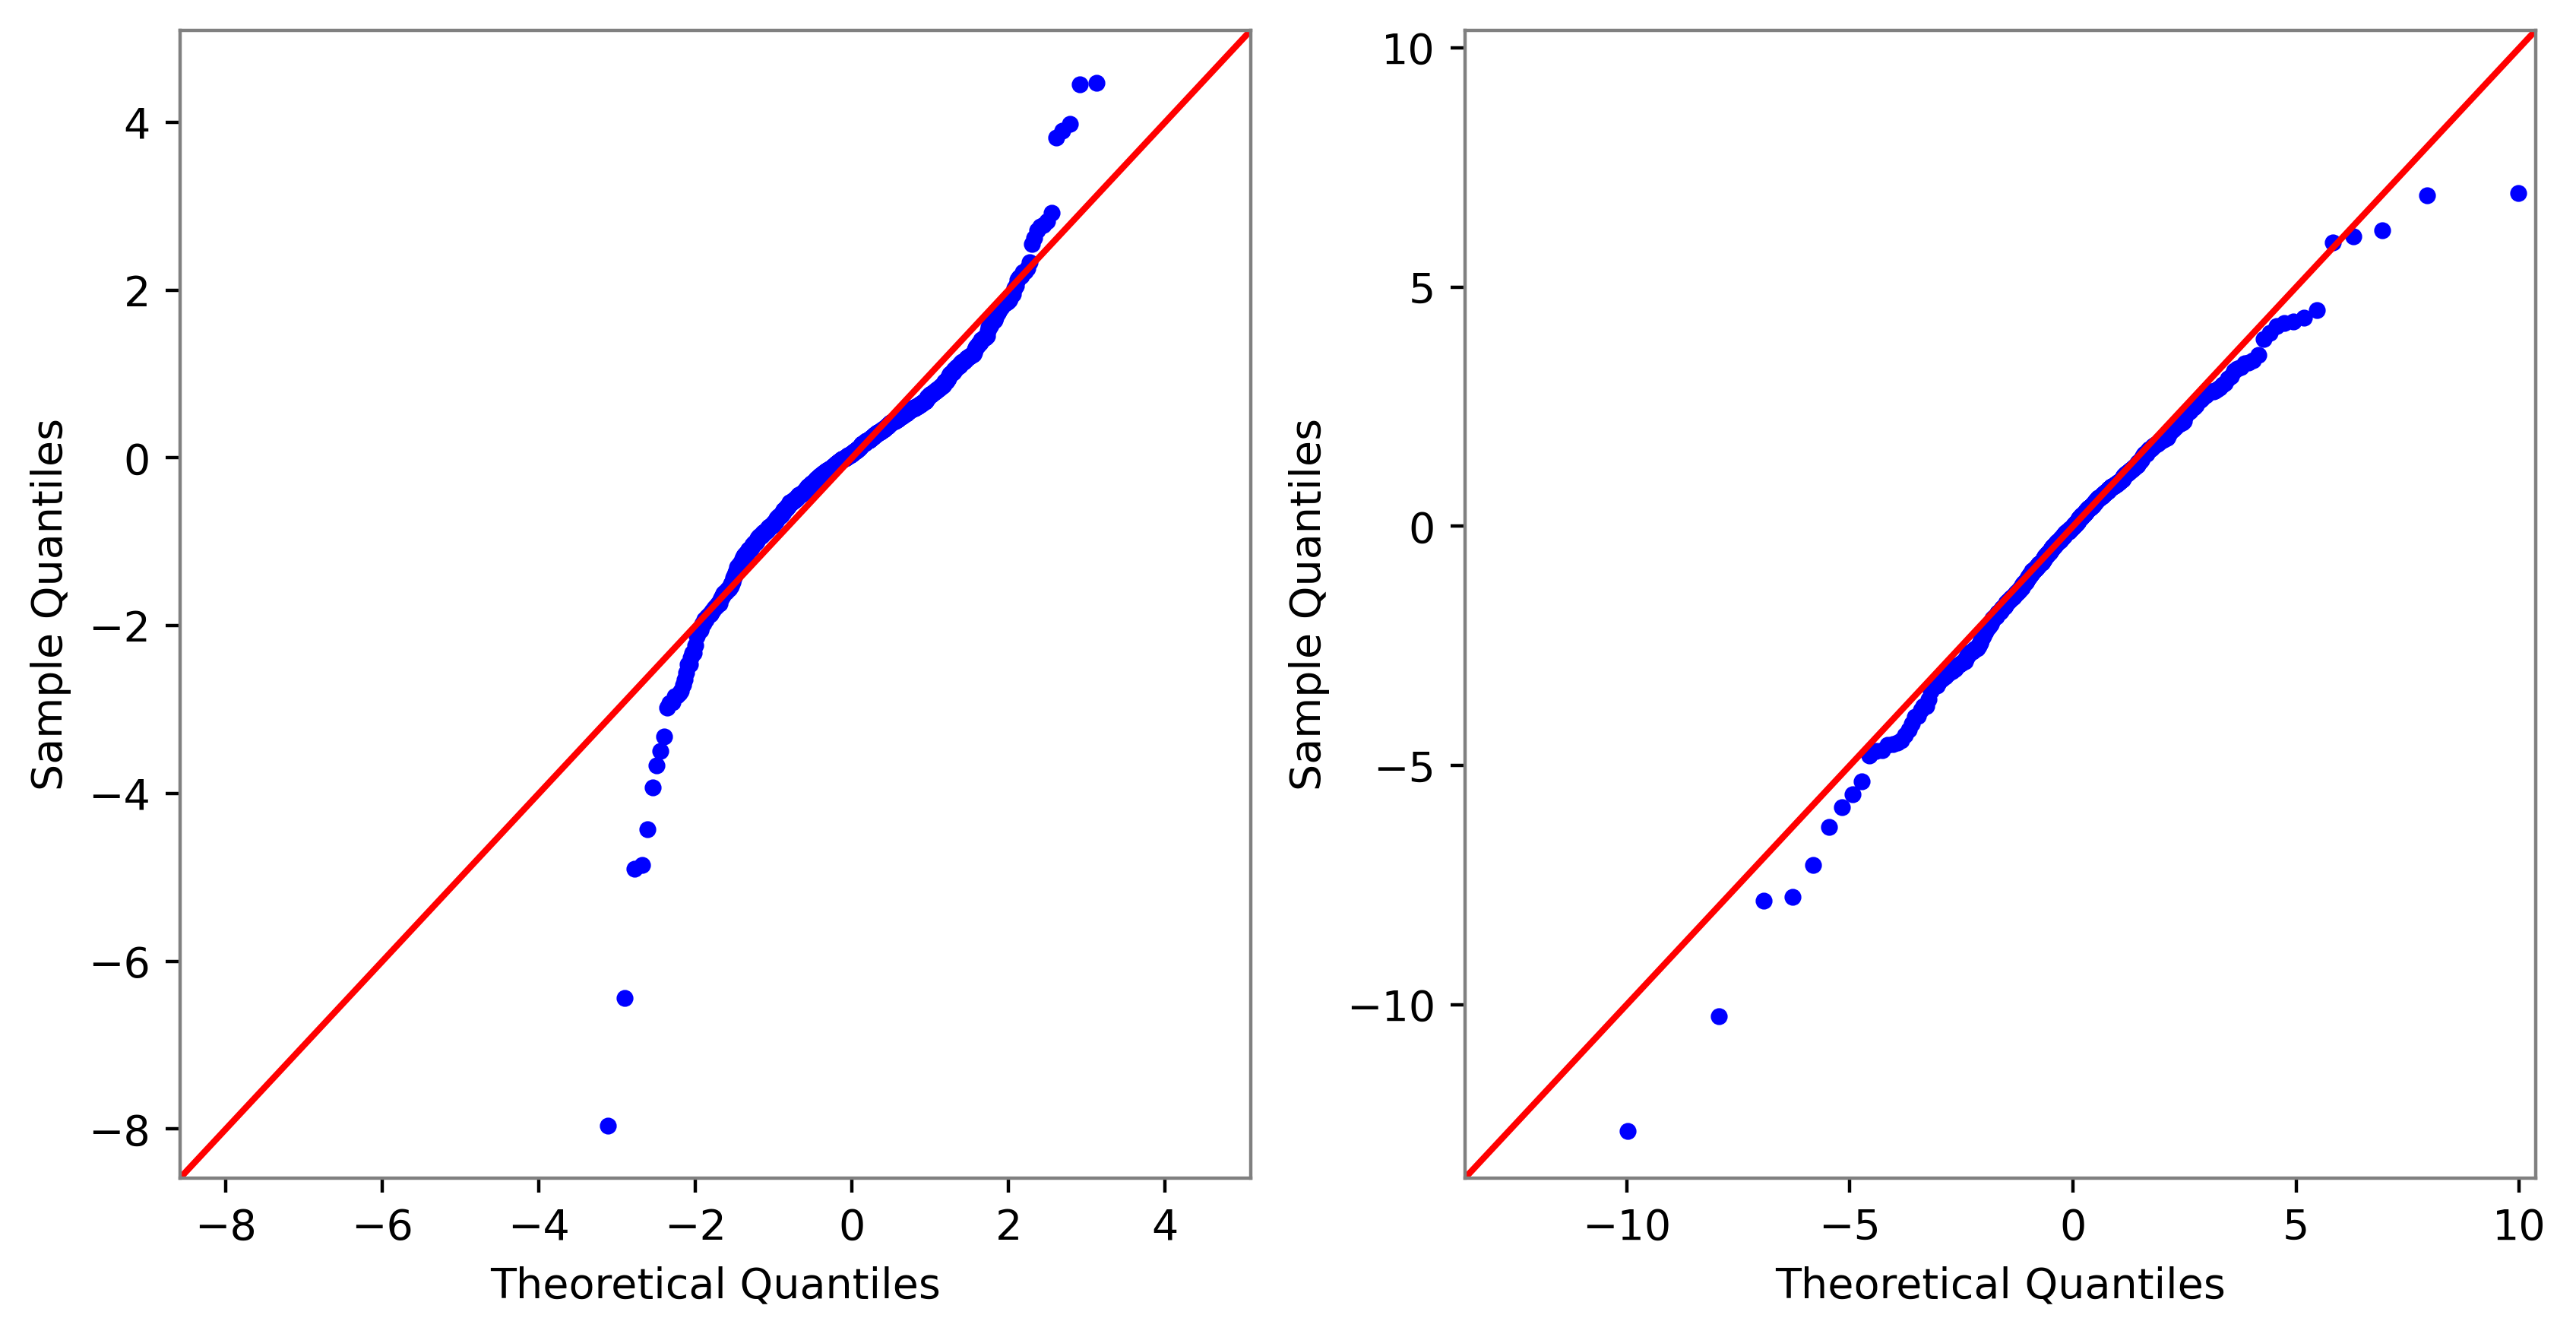
\includegraphics[width=3.5in]{figures/qqplot_sp.png}
        \caption{Q-Q plots of S\&P 500 index weekly return. The parametric curve is generated by different distributions (left: normal distribution, right: t-distribution with degree of freedom equals to 3). From the figure, we can conclude the fat tail characteristics of the S\&P 500 index weekly return.}
        \label{fig:qqplot_sp}
    \end{figure}
    
         \begin{figure}[h]
        \centering
        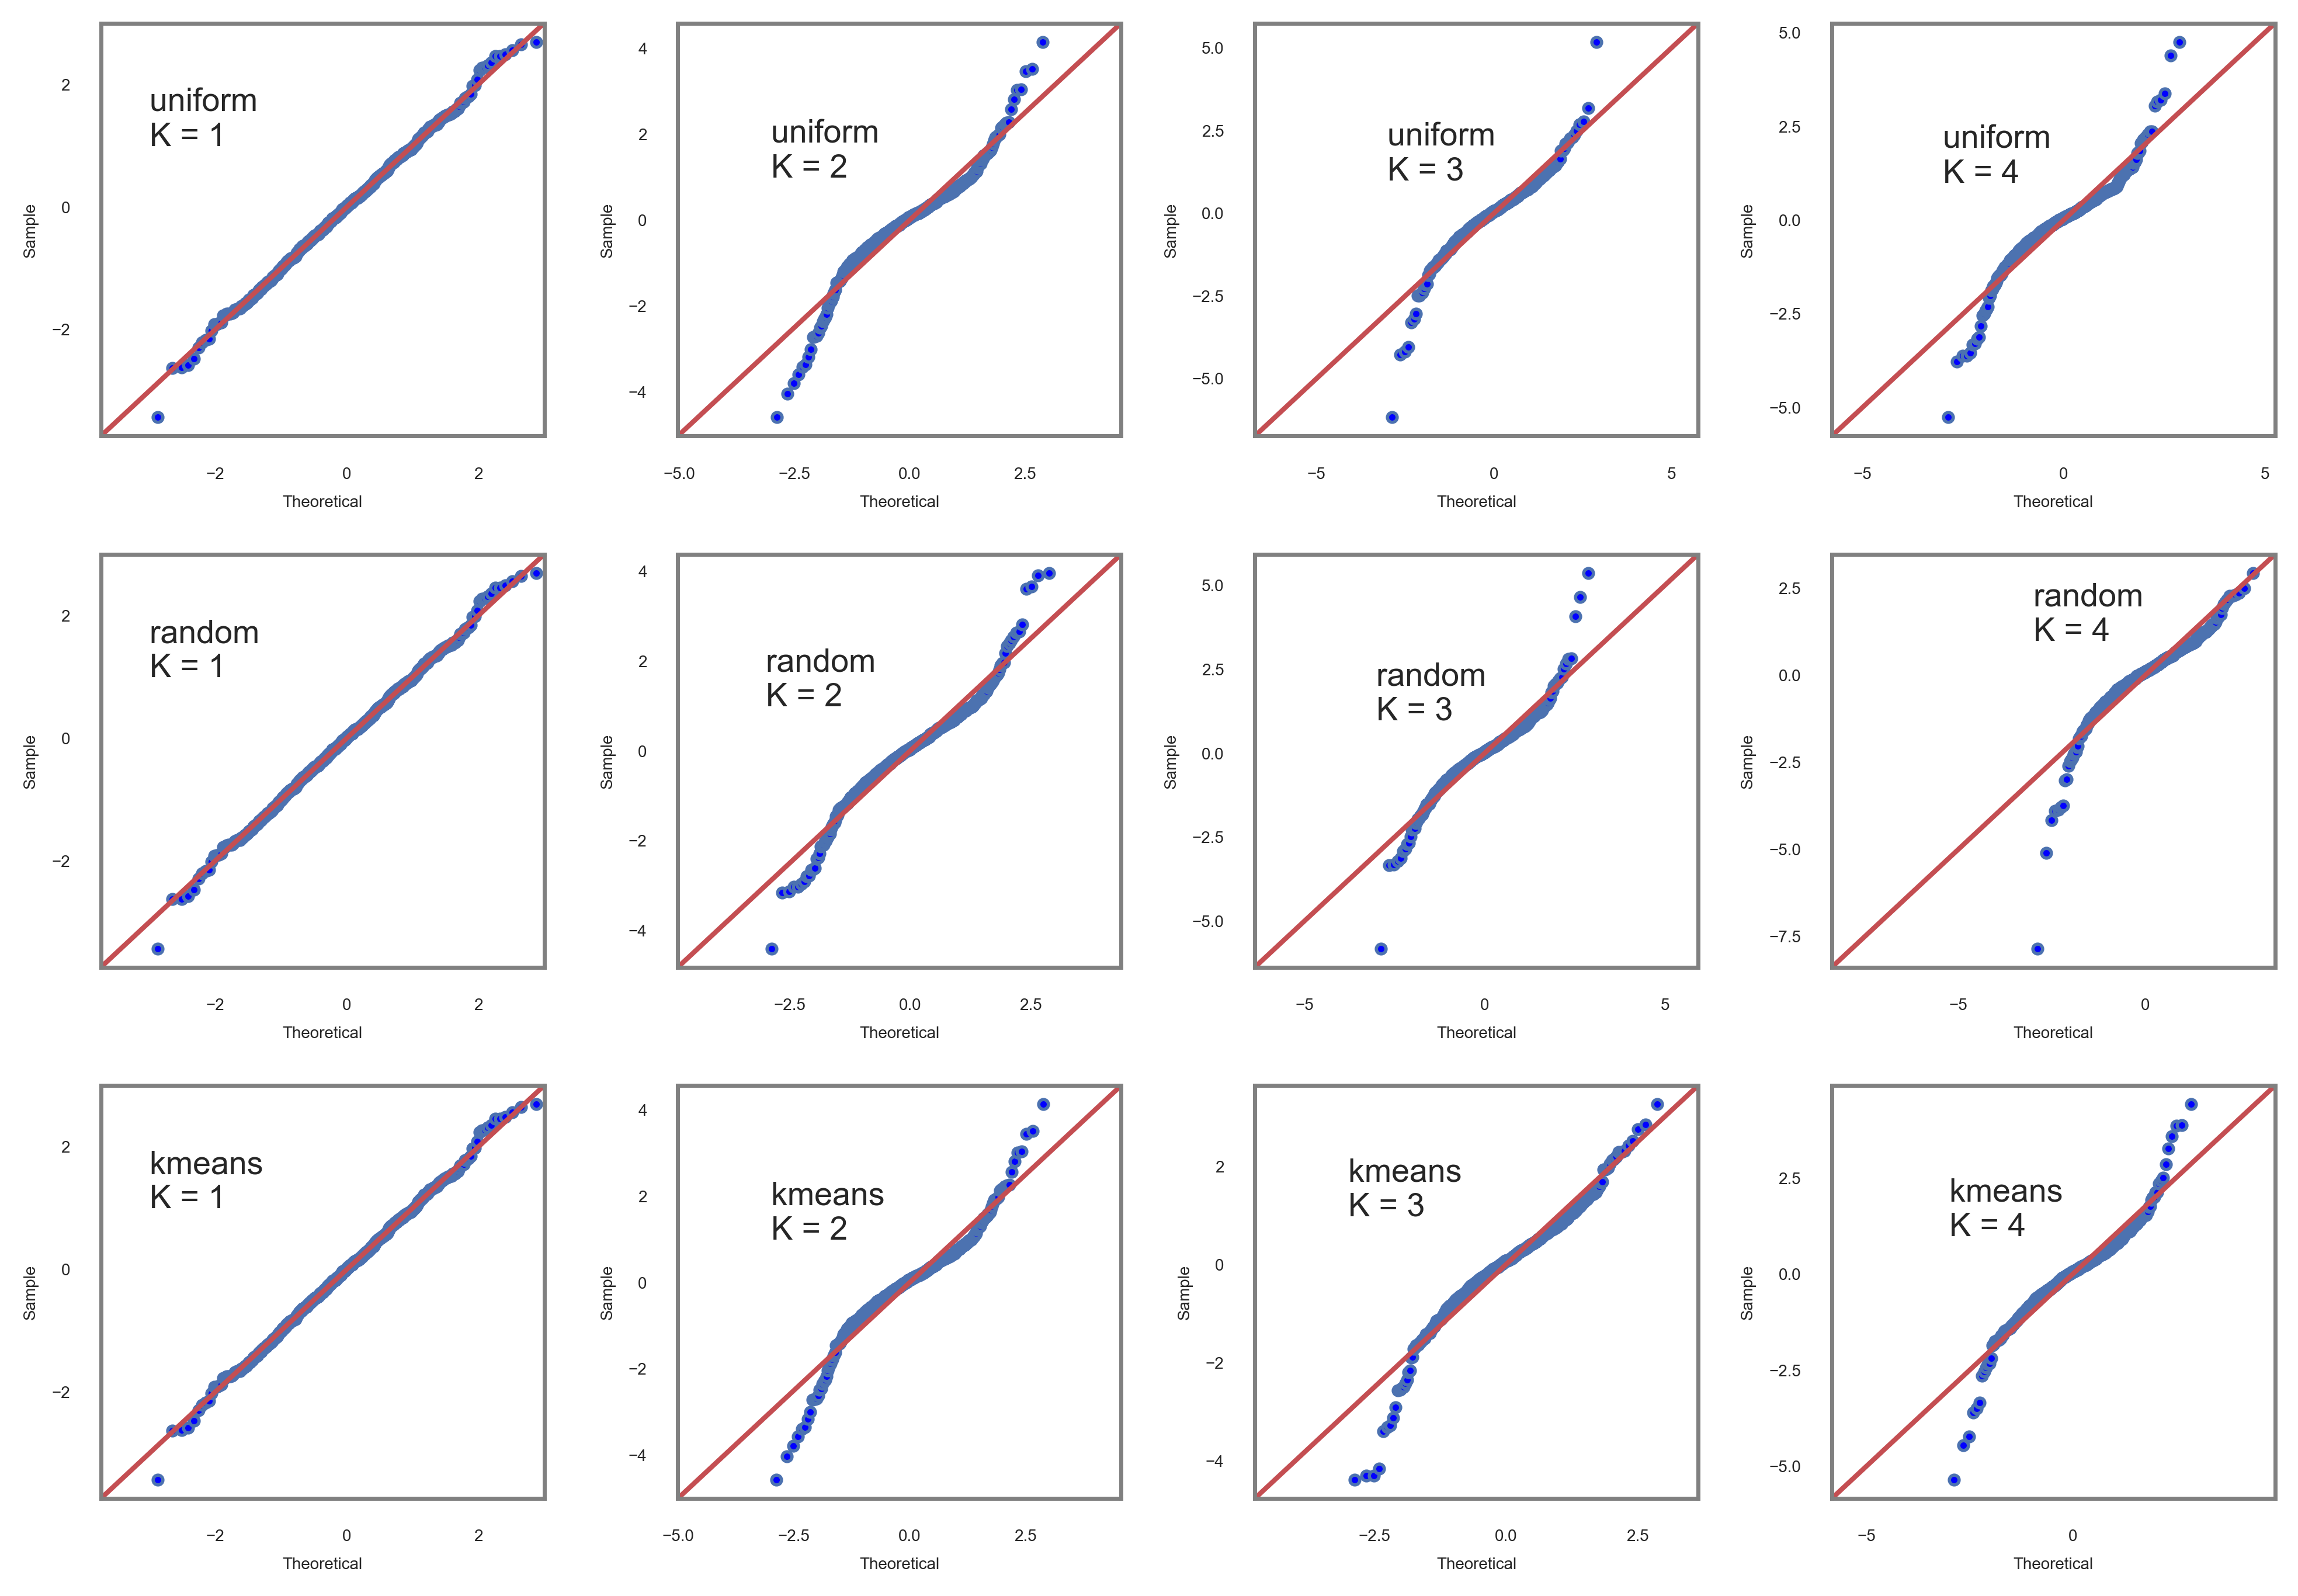
\includegraphics[width=3.5in]{figures/qqplot.png}
        \caption{Q-Q plots of GMM fitted S\&P with different initialization methods (Uniform Distribution Sampling, Random Sampling, K-means) and number of components (1$\sim$4). (horizontal: sample quantile, vertical: theoretical quantile). If we only used one component in the GMM model, the fitted distribution is also normal. When we used more than one components, the Q-Q plots all show similar fat tail pattern no matter what initialization methods we used.}
        \label{fig:qqplot}
    \end{figure}
    
    
    We also compared the histogram and the density functions fitted by kernel density estimation and GMM respectively in Figure \ref{fig:hist_GMM}. In the zoomed view of the tail, we can see that GMM can't fit the density well. The tail of the fitted GMM density is thinner than that of the kernel density.
    
    All of this evidence shows that GMM can capture a part of tail risk near the tail part but fail to reproduce correctly the fat tail of S\&P index returns. (\textbf{RQ4}) 
    
    

    %To further explore whether the GMM model is able to reproduce correctly the fat tail of S\&P, our answer is NO. 
    %Furthermore, as is suggested by Figure \ref{fig:log_plot_tail} that GMM's fitting ability on S\&P 500 index curve degenerates as the quantile goes towards 1, we can prove GMM decays faster than S\&P 500 index mathematically.    
    %we compared the fitted GMM density and the histogram of the original data. From the figure, we can also see that the fitted GMM density decays at the tail and thus fails to correctly reproduce those extreme returns. Therefore, the GMM model is unable to reproduce correctly the tails of the S\&P 500 index density.
    
     \begin{figure}[h]
        \centering
        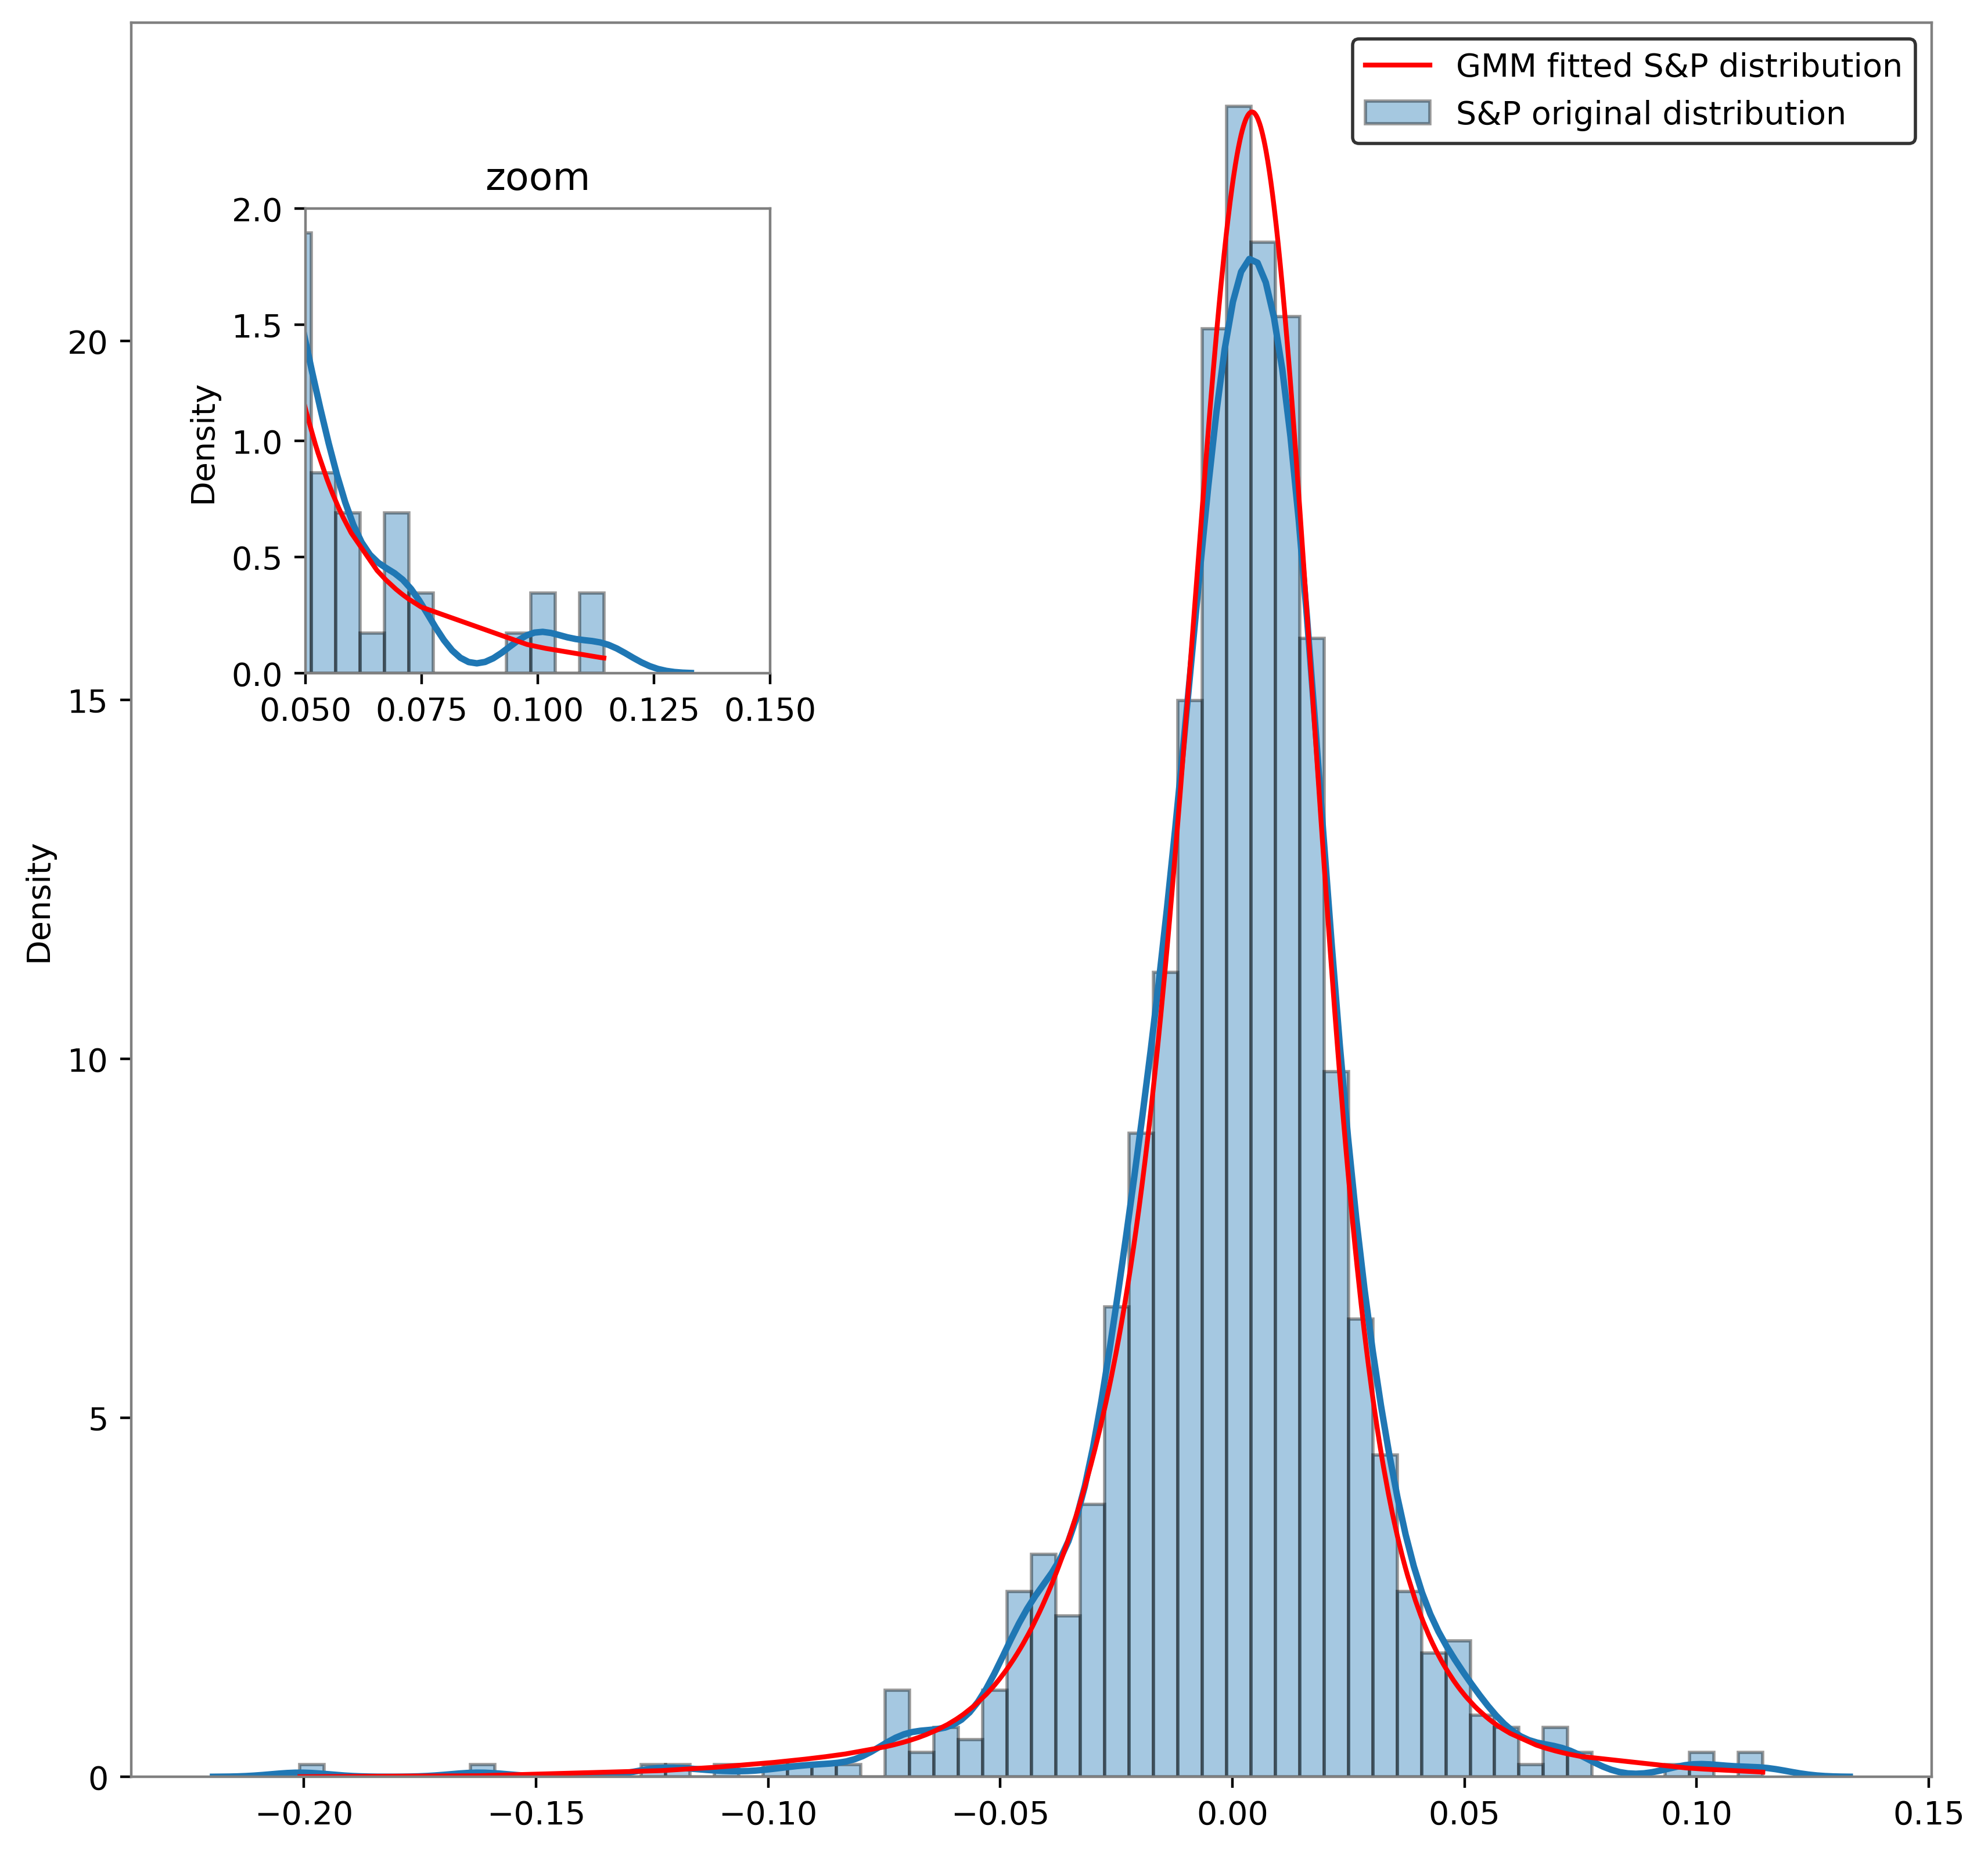
\includegraphics[width=3.5in]{figures/hist_GMM.png}
        \caption{GMM fitted results and S\&P histogram with zoomed view on the tail distribution. In the zoomed view of the tail, we can see that the tail of the fitted GMM density is thinner than that of the kernel density. }
        \label{fig:hist_GMM}
    \end{figure}
    
    
    \subsubsection{LapGMM for Two Moons Example}
    From Figure \ref{fig:lapgmm}, we can see that LapGMM successfully identifies the moon clusters, which proves its ability to have complex decision boundaries, in contrast to linear decision boundaries of K-means, and quadratic decision boundaries of standard GMM. This is mainly contributed by the regularization term $\sum_{k}\mathcal{R}_k$, which can also answer \textbf{RQ5}. To further see how LapGMM improves its estimation throughout iterations, we plotted the evolution of objective function $\mathcal{L}(\Theta)$, log-likelihood function $\mathcal{Q}(\Theta, \Theta^{n-1})$, regularization term $\sum_{k}\mathcal{R}_k$ and accuracy, as shown in Figure \ref{fig:loss} and \ref{fig:acc}.
    
    \begin{figure*}[!t]
        \begin{subfigure}{.23\textwidth}
            \centering
            % include first image
            \vspace{1ex}
            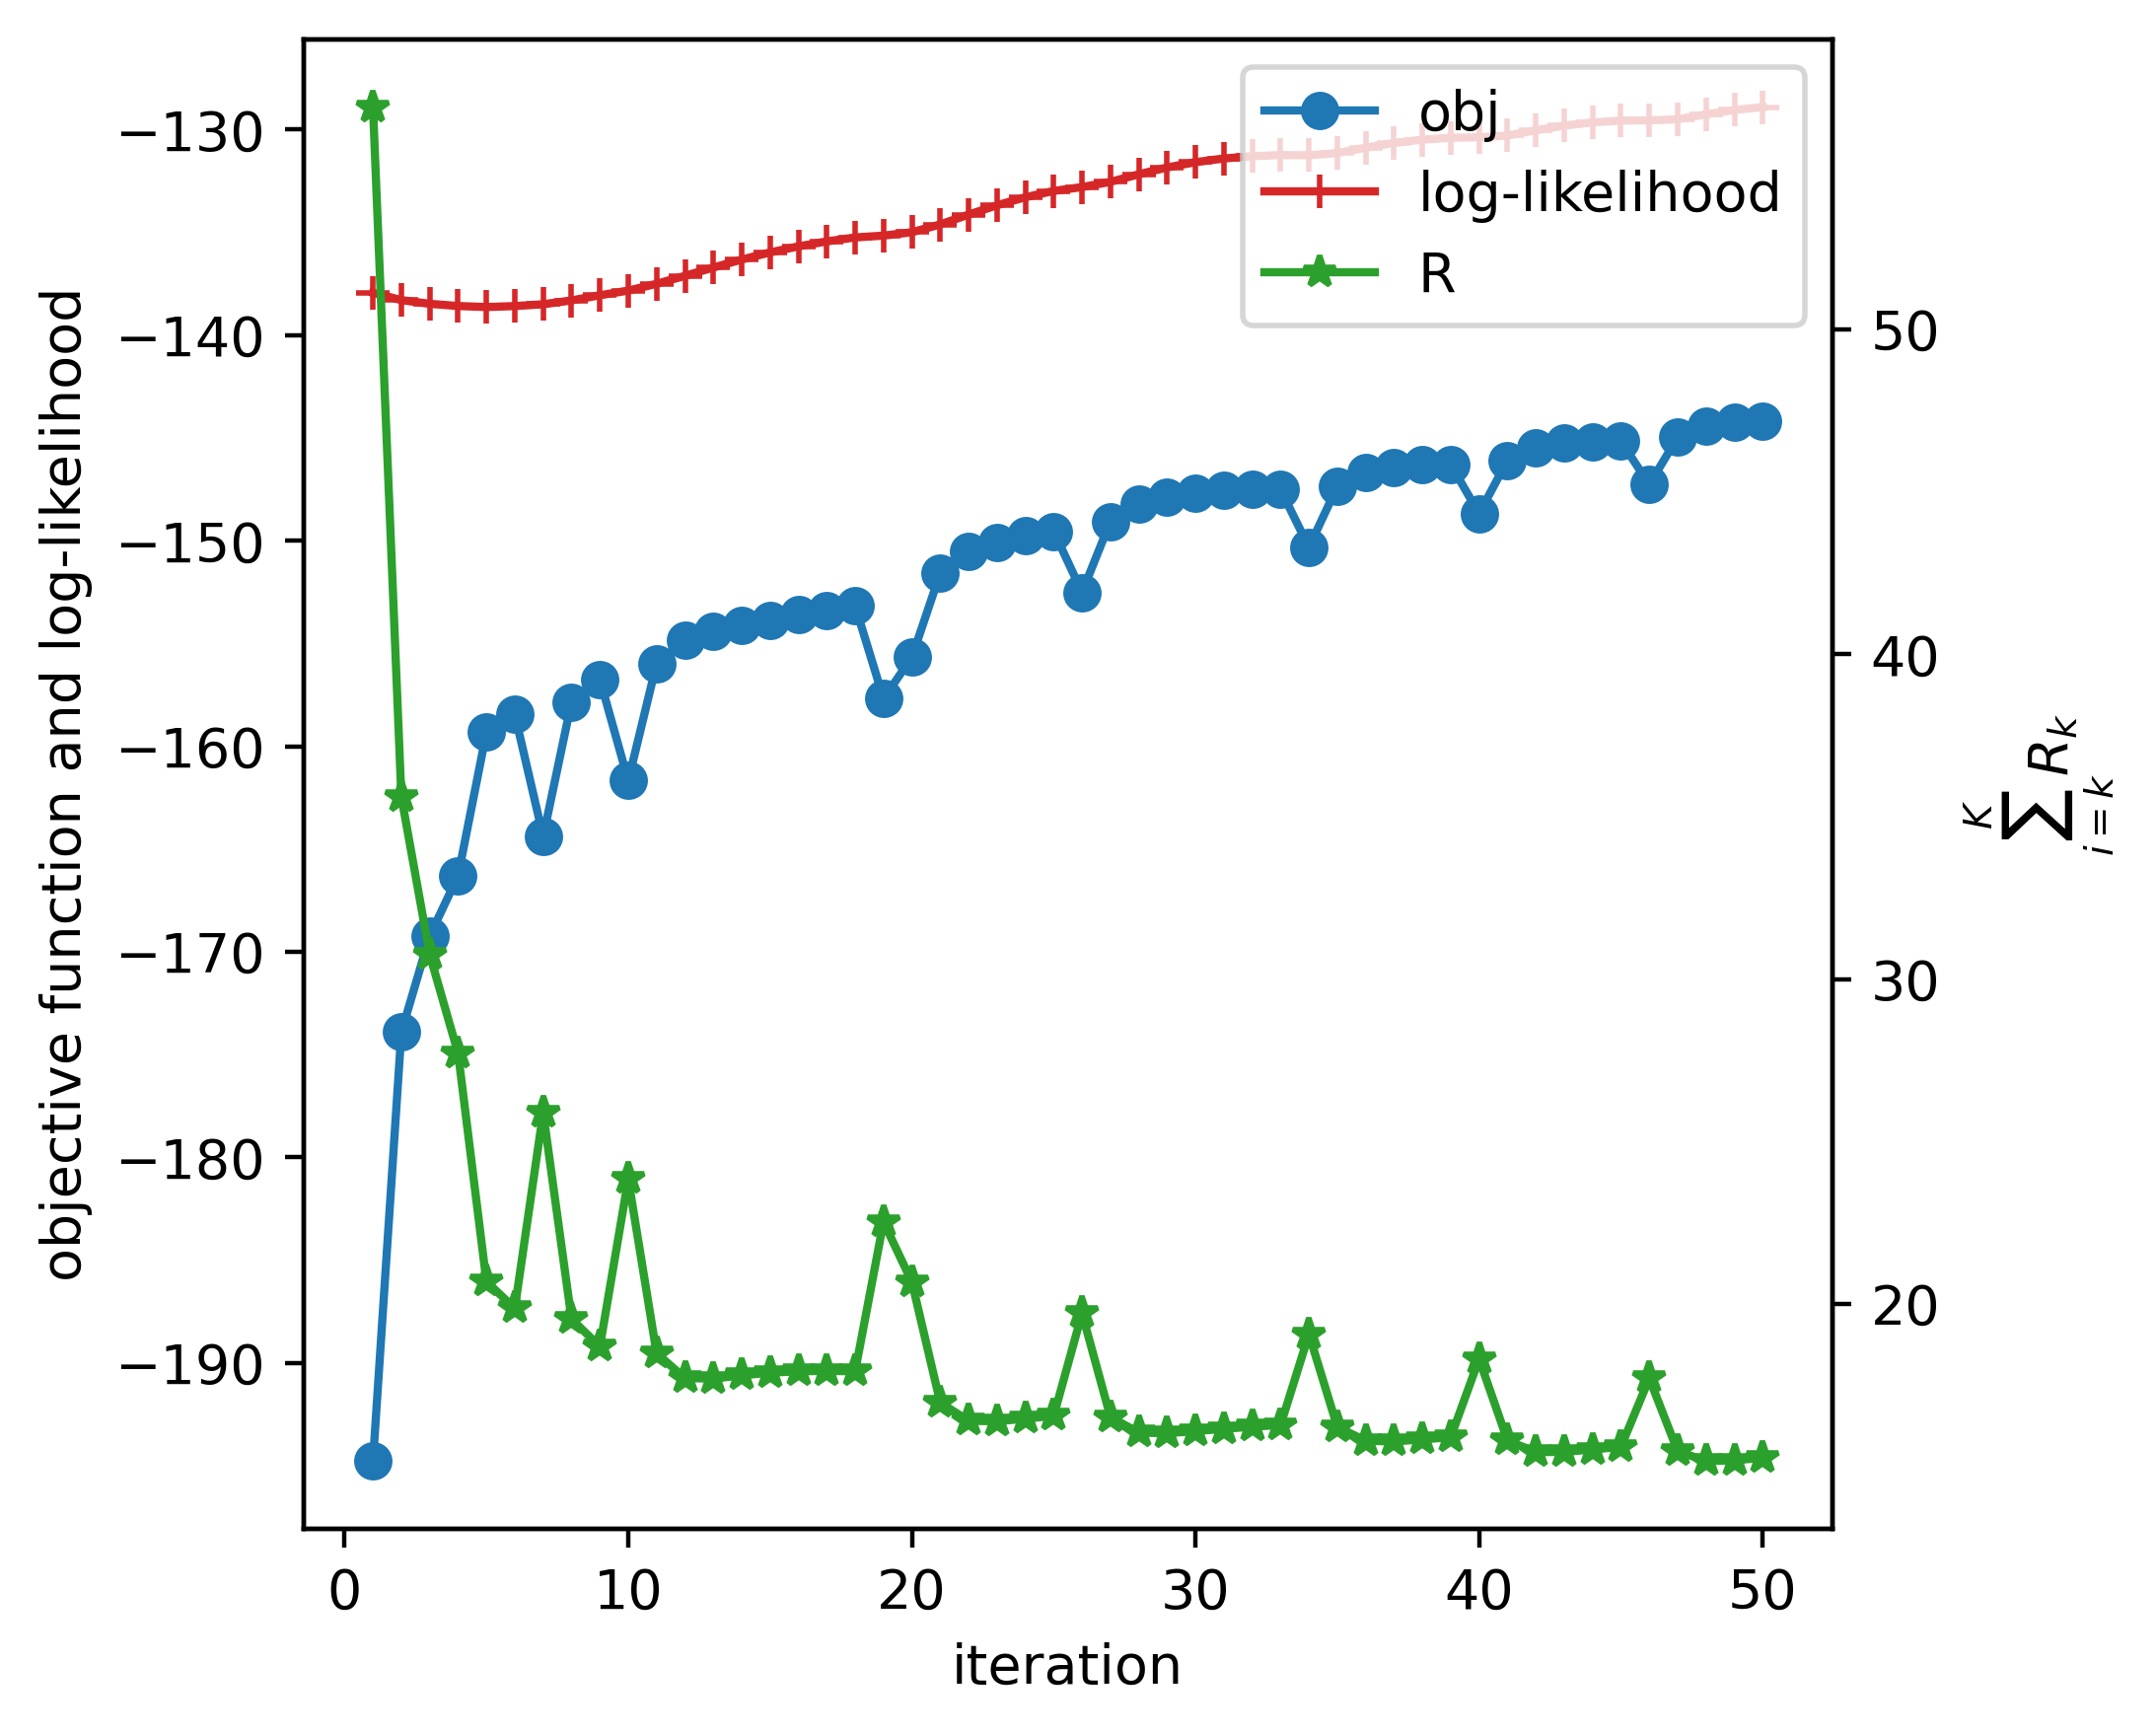
\includegraphics[width=1.15\linewidth]{figures/loss.png}  
            \caption{\vspace{1ex}Objective evolution}
            \label{fig:loss}
        \end{subfigure}
        \hspace{5ex}
        \begin{subfigure}{.23\textwidth}
            \centering
            % include first image
            \vspace{1ex}
            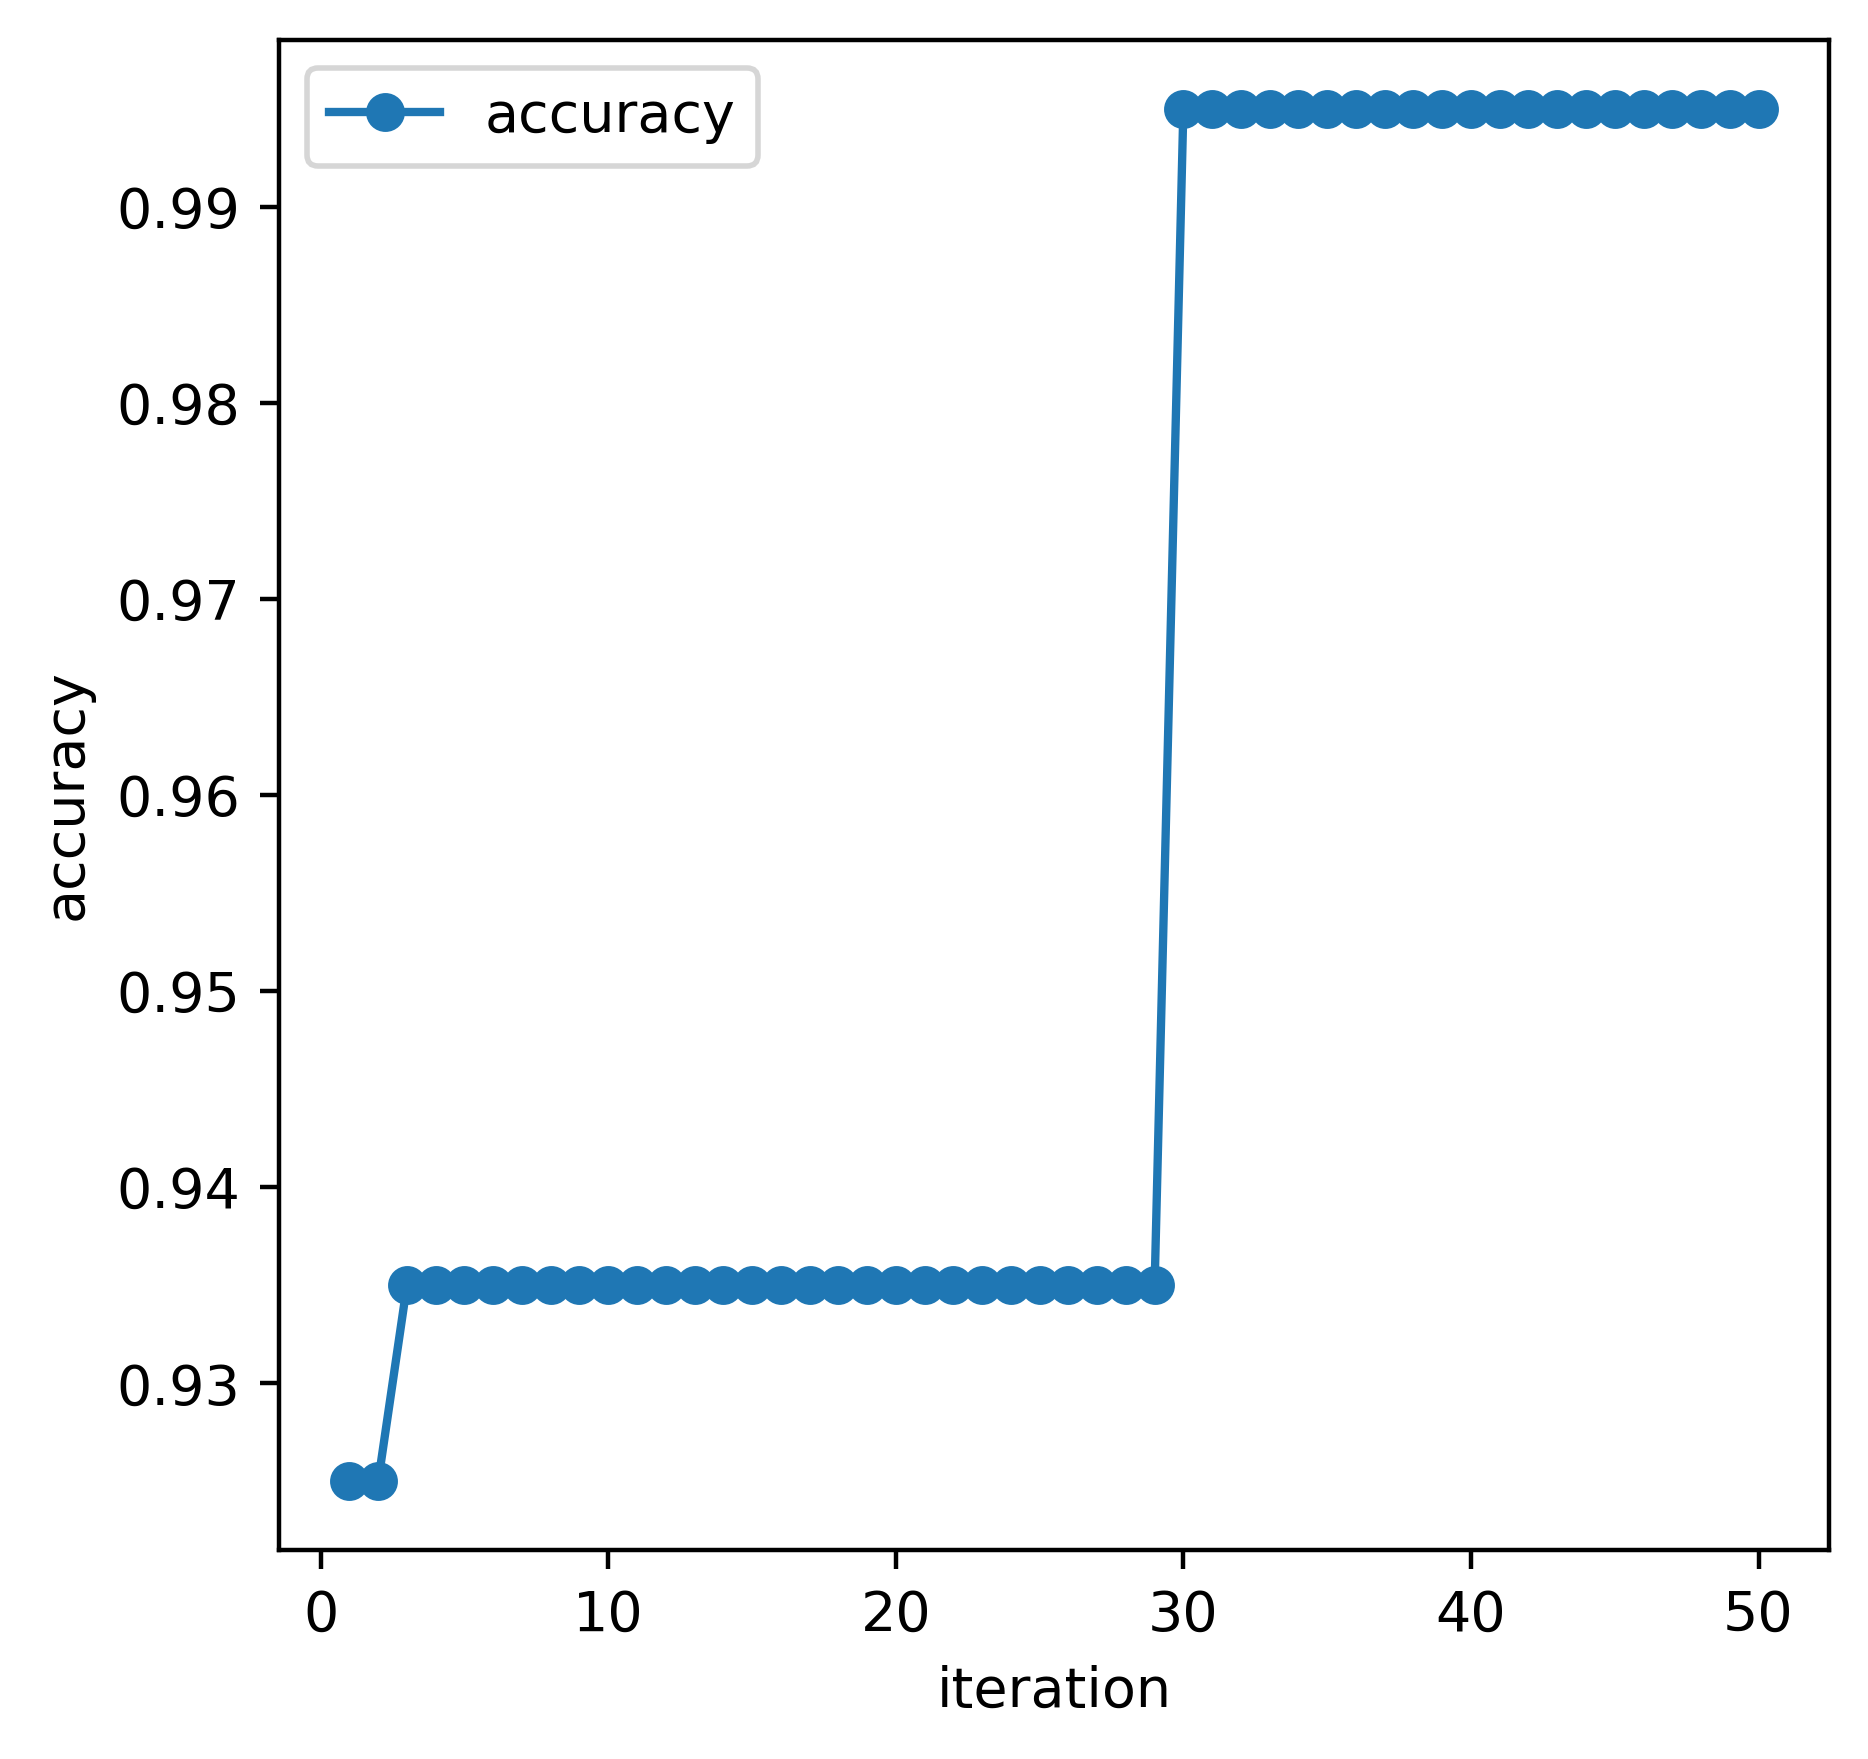
\includegraphics[width=\linewidth]{figures/acc.png}  
            \caption{Accuracy evolution}
            \label{fig:acc}
        \end{subfigure}
        \begin{subfigure}{.23\textwidth}
            \centering
            % include first image
            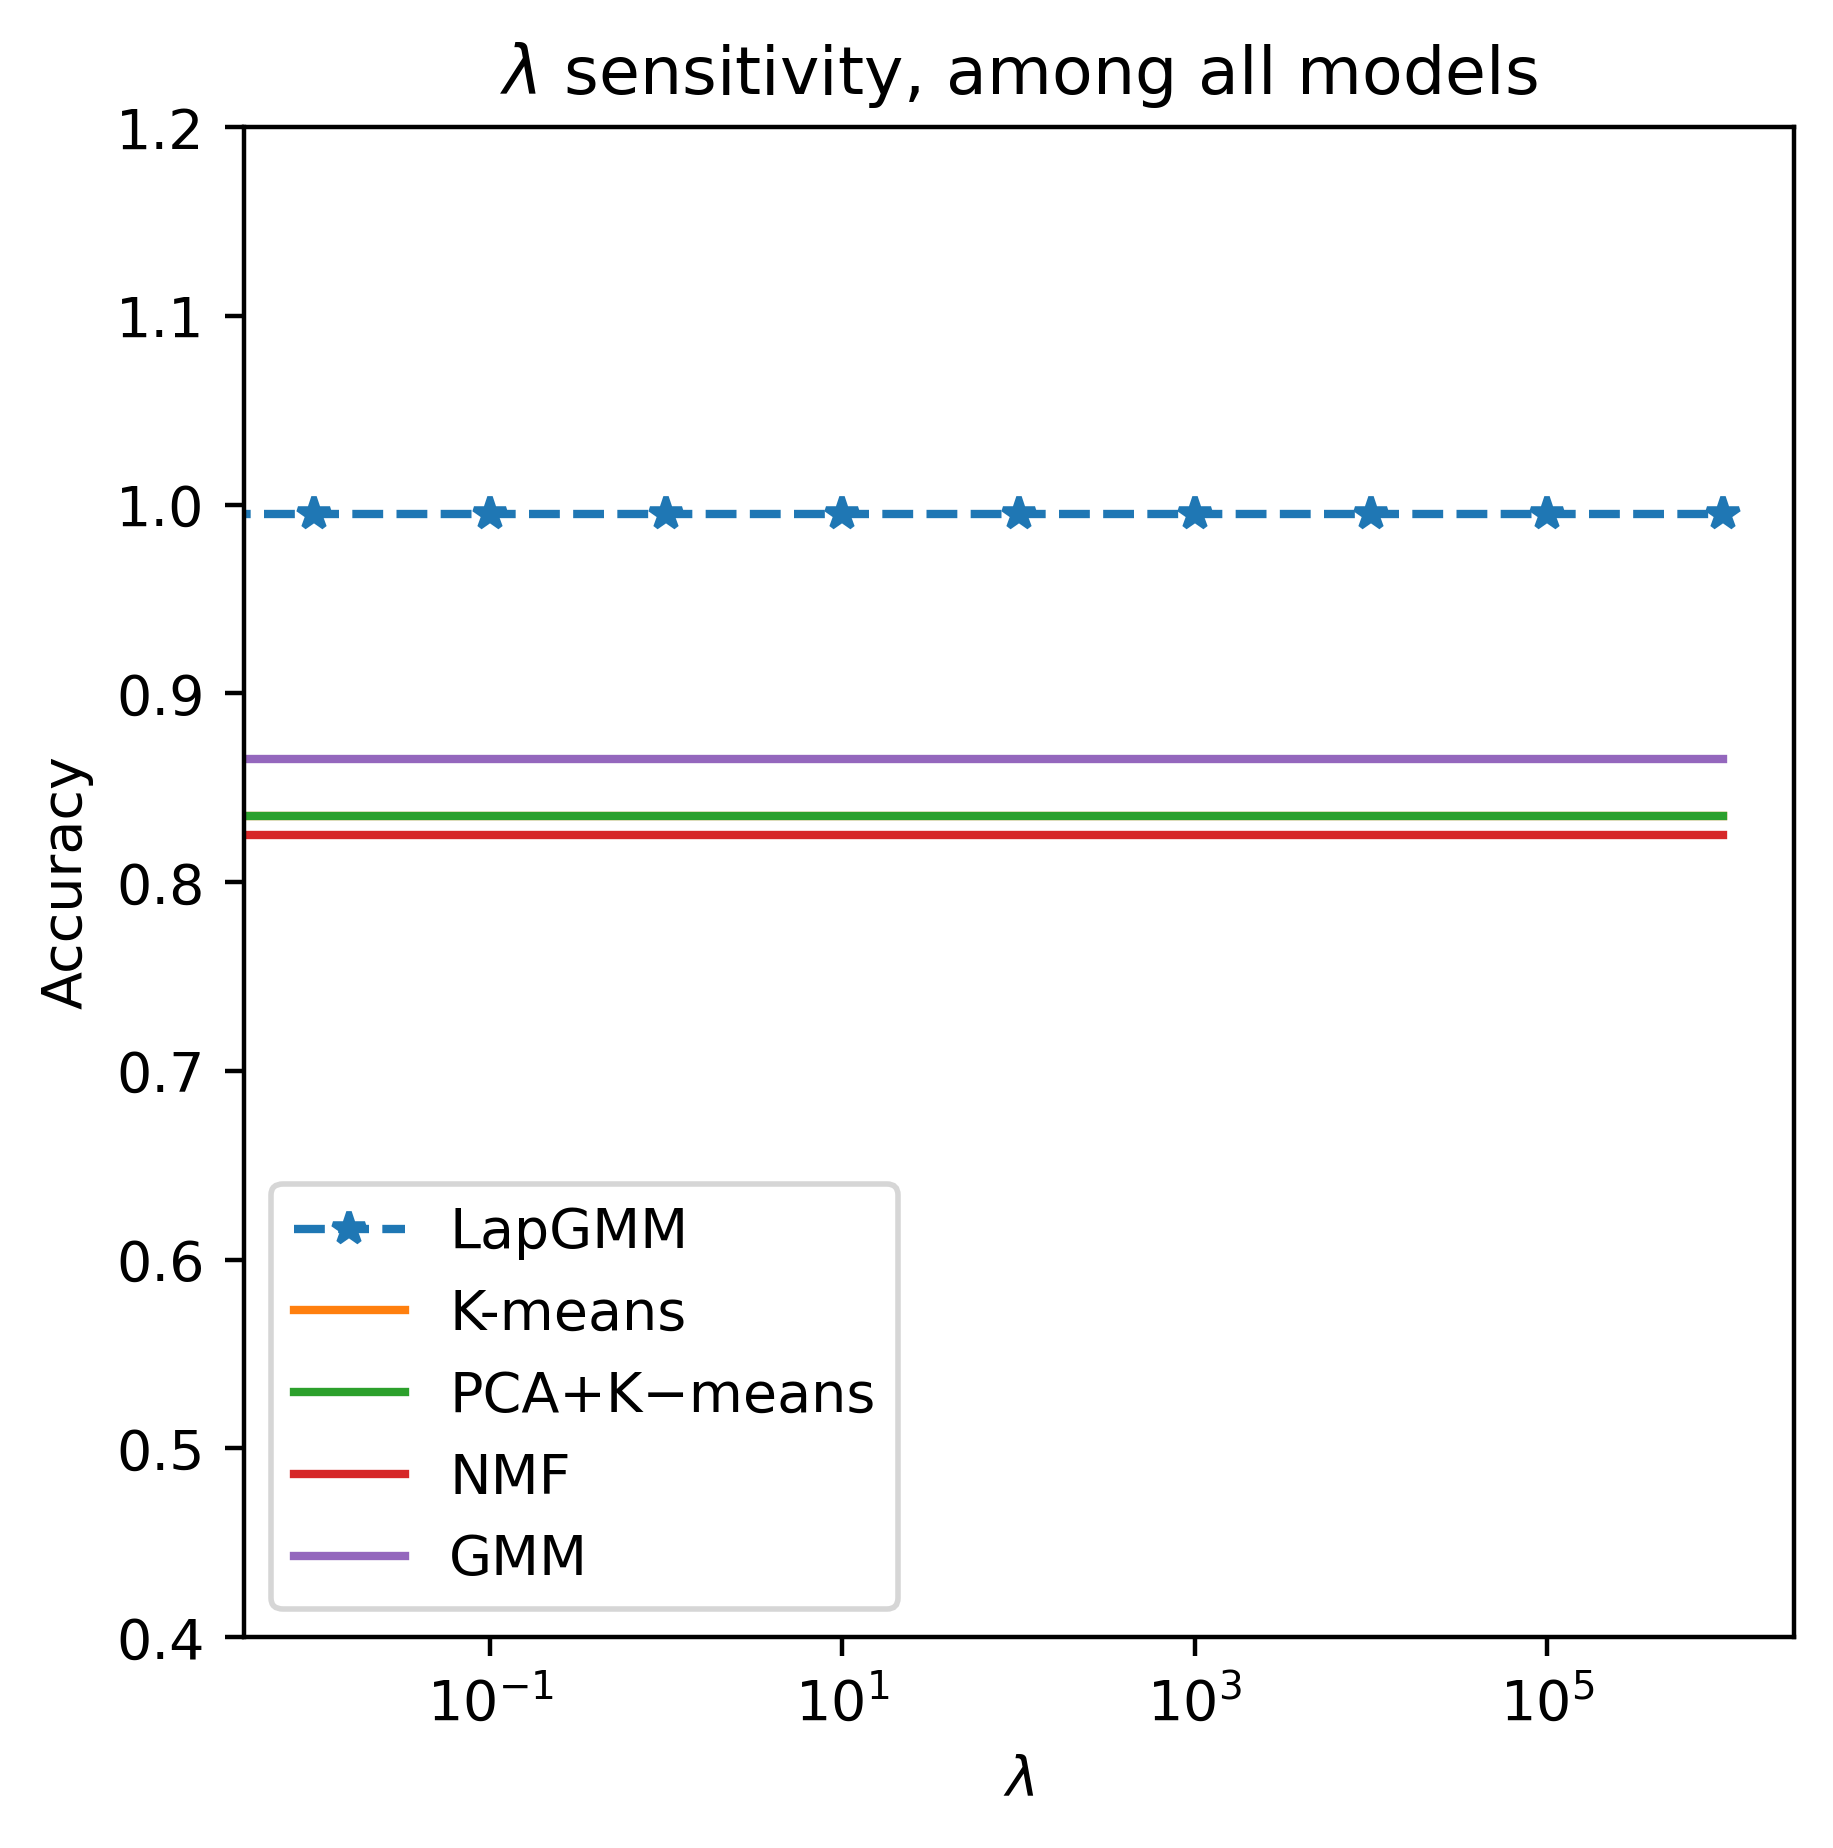
\includegraphics[width=\linewidth]{figures/lambda.png}  
            \caption{Sensitivity w.r.t. $\lambda$}
            \label{fig:lambda}
        \end{subfigure}
        \begin{subfigure}{.23\textwidth}
            \centering
            % include first image
            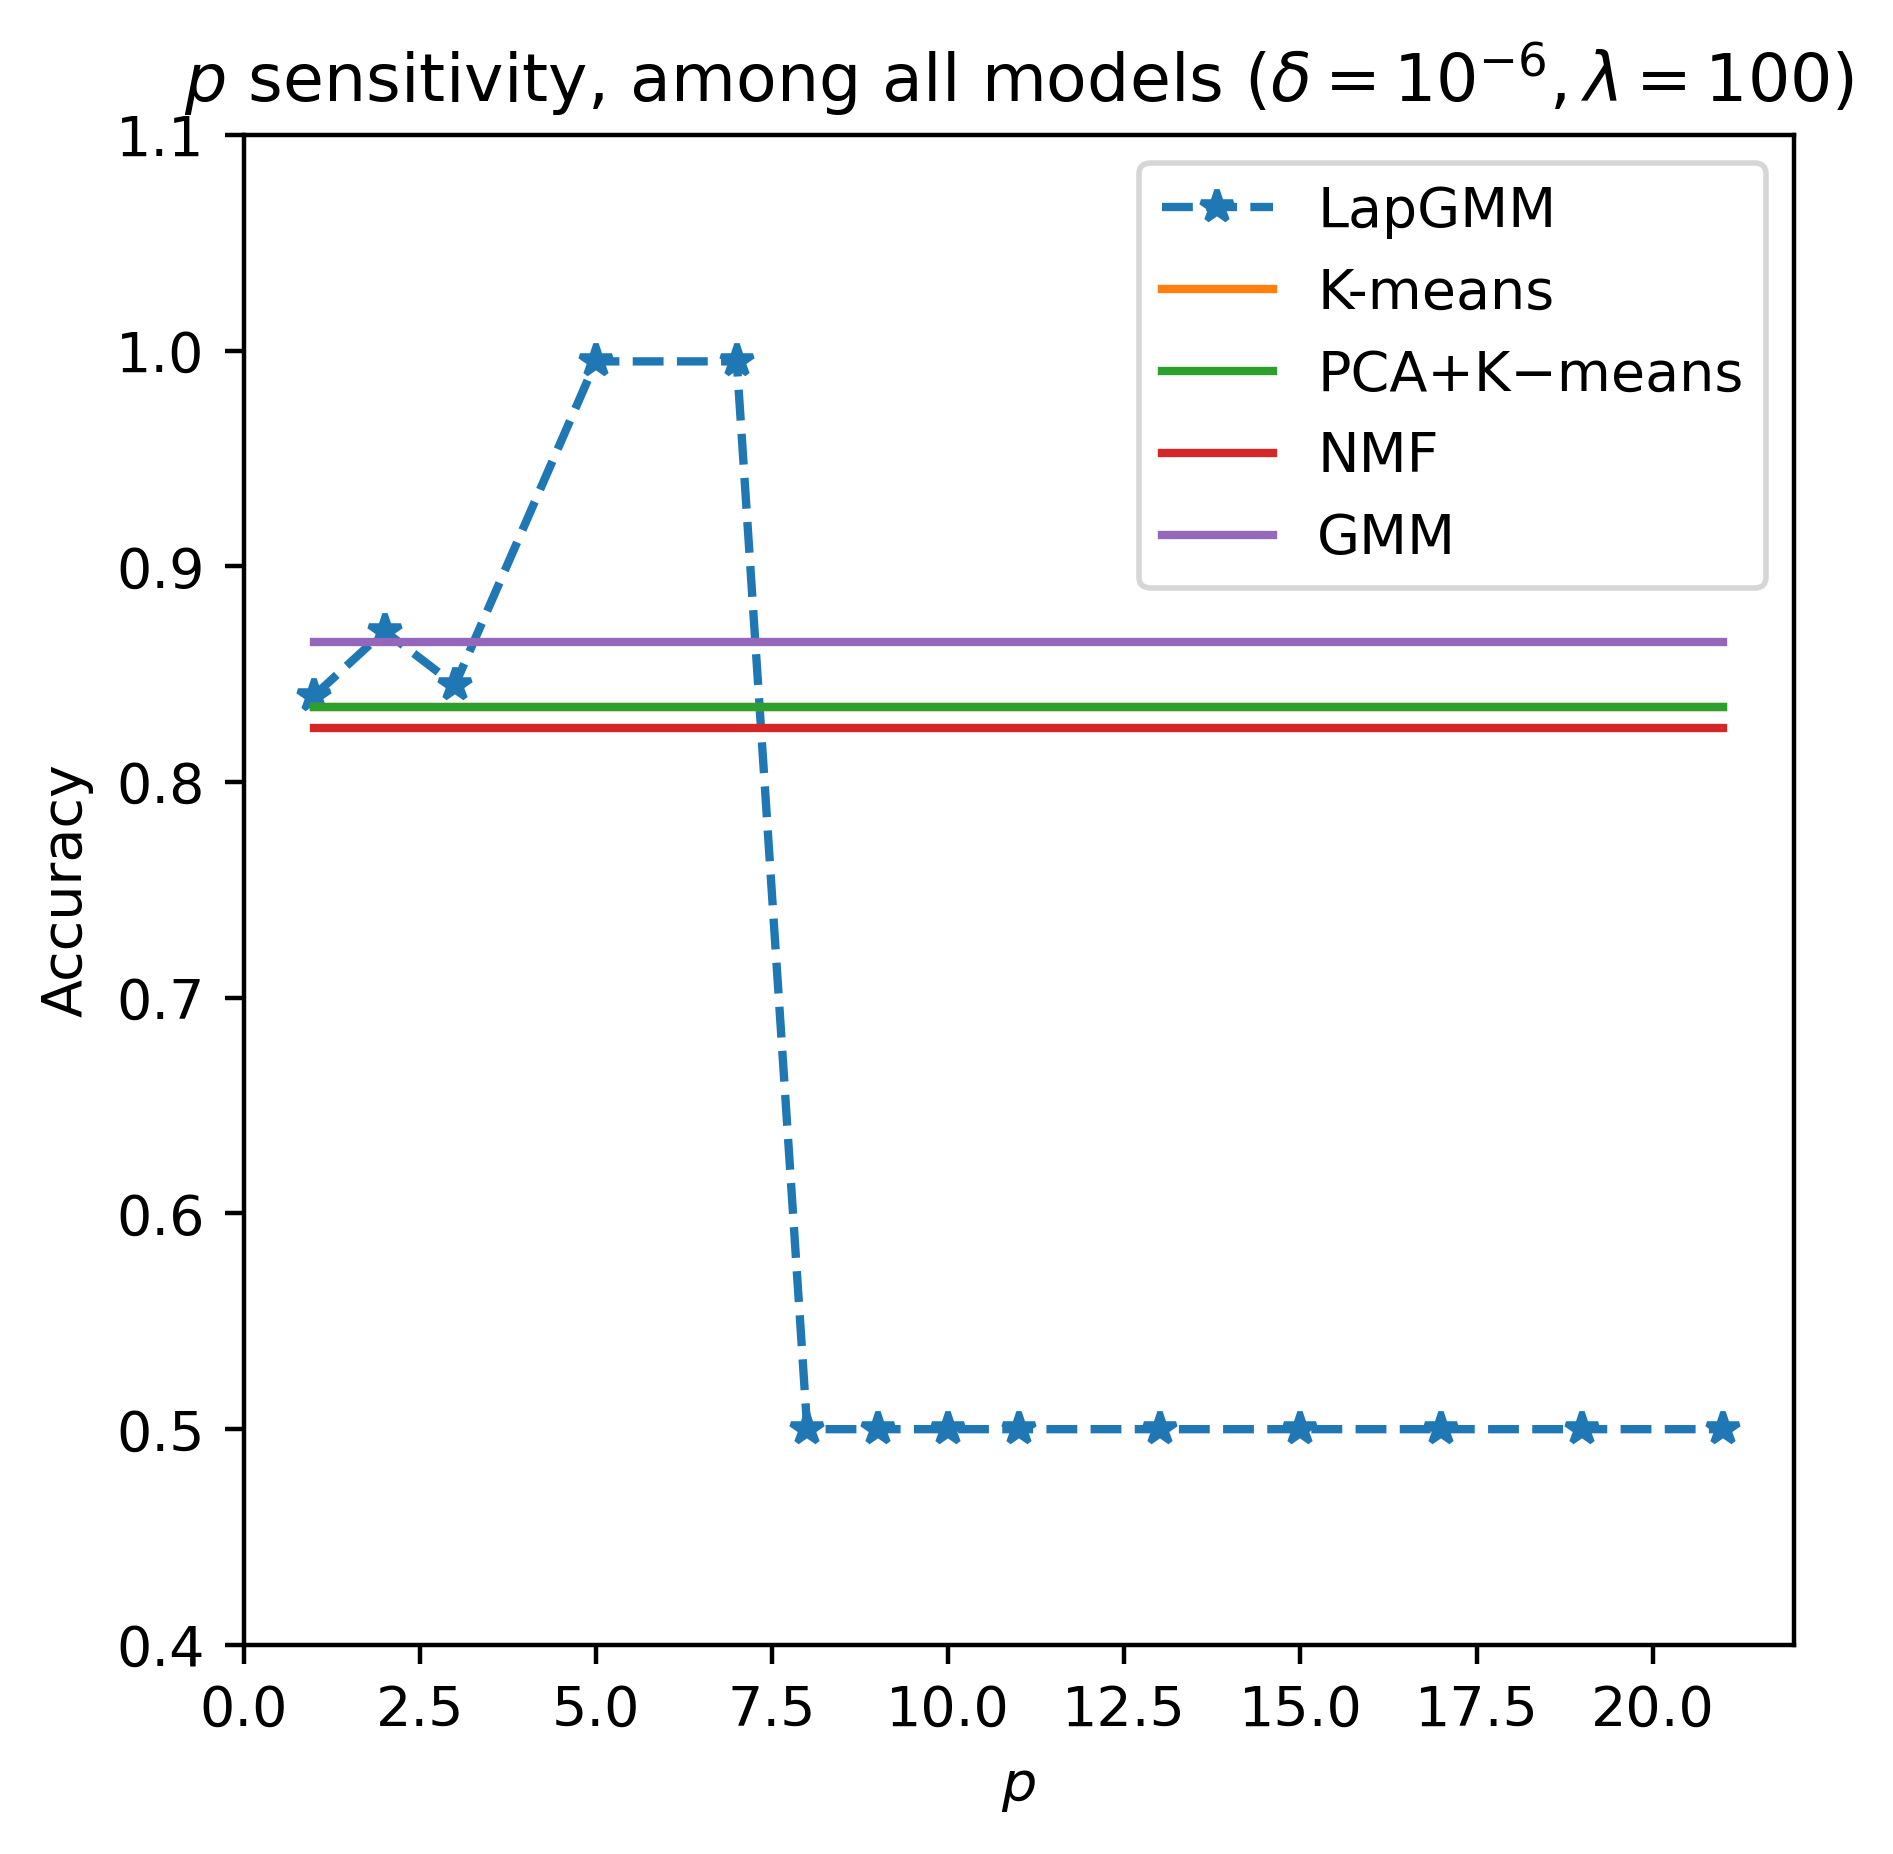
\includegraphics[width=\linewidth]{figures/p.png}  
            \caption{Sensitivity w.r.t. $p$}
            \label{fig:p}
        \end{subfigure}
        \caption{(a) -- (b) Evolution of objective function $\mathcal{L}(\Theta)$, log-likelihood function $\mathcal{Q}(\Theta, \Theta^{n-1})$, regularization term $\sum_{k}\mathcal{R}_k$ and accuracy, throughout all iterations. As we can see once the regularization term is small enough, the accuracy will jump to a high level. (c)-- (d) Performance sensitivity of LapGMM, K-means, PCA + K-means, NMF and standard GMM, w.r.t changes in $\lambda$ and $p$.}
    \end{figure*}

    We could see that $\mathcal{Q}(\Theta, \Theta^{n-1})$ continuously increases, while $\sum_{k}\mathcal{R}_k$ does not. In each iteration, LapGMM maximizes log likelihood and minimizes manifold regularization respectively using Newton's method, to find a "locally better" fit for the parameters. Therefore, if stopping criteria of Newton’s method are too strict in M-step, it will more likely find a globally optimal $\Theta$, causing a jump in $|f_k(\x_i) - f_k(\x_j)|$ if $\x_i$ and $\x_j$ are “close”, as well as a jump in $\sum_{k}\mathcal{R}_k$.
    
    While tuning the definition of weight matrix $S$, the regularization coefficient $\lambda$, the number of nearest neighbors $p$, and the maximum number of iterations $N$, LapGMM’s performance varies a lot. See Figure \ref{fig:S-p} for an example of LapGMM’s performance robustness, w.r.t. different $S$ and $p$ respectively. Notice that sometimes the LapGMM clusters all data points into a single cluster. This is a typical overfitting phenomenon with respect to $\sum_k \mathcal{R}_k$. We can easily find that $\Prob(k | \x) = 1/K$ will make the regularization $0$ which happens to be the global minimum. Thus if we over smooth the posterior in the Newton method step, we will get a very small regularization term. That corresponds to a posterior probability of $0.5$ for all the data points. Thus we need to control the $\delta_{\mathrm{NR}}, N_{\mathrm{NR}}$ to avoid overfitting.
    
    \begin{figure}[t]
        \centering
        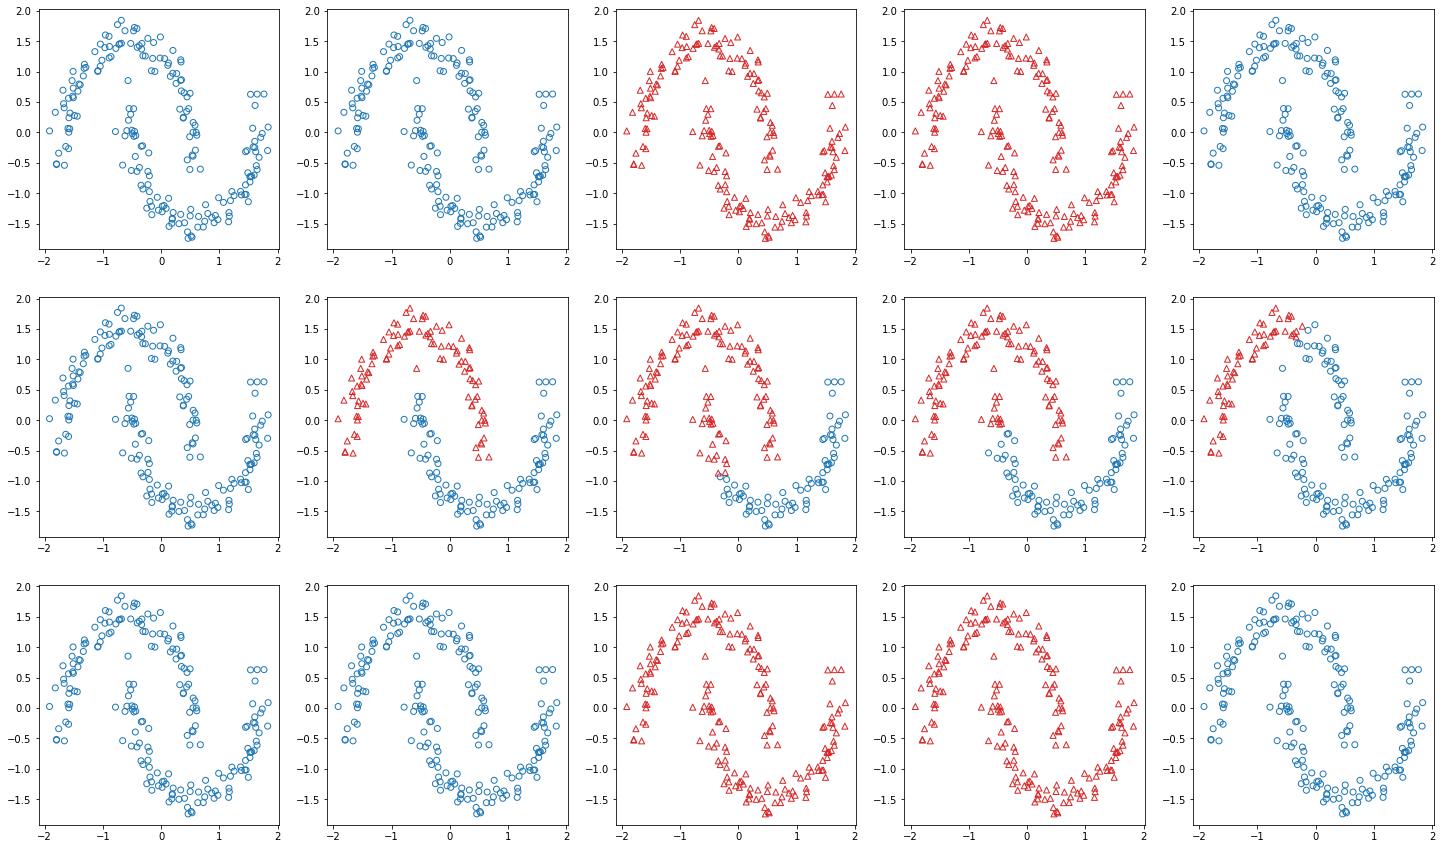
\includegraphics[width=0.45\textwidth]{figures/LapGMMrobustnessSp.png}
        \caption{Performance robustness of LapGMM, w.r.t $S$ and $p$; row 1$\sim$3 for $S\in\{\mathrm{'0-1'},\mathrm{'dot-product'},\mathrm{'heat'}\}$; column 1$\sim$5 for $p\in\{8,7,6,5,4\}$. As we can see if we change the weight matrix $S$, the performance of LapGMM will change by a lot.}
        \label{fig:S-p}
    \end{figure}
    
    LapGMM outperforms other clustering algorithms, with “good” hyper-parameters. From Figure \ref{fig:lambda} and \ref{fig:p}, we can also see that LapGMM generally outperforms other clustering algorithms, including K-means, PCA + K-means, NMF and standard GMM. 
    In addition, the performance of LapGMM is not affected by changes in $\lambda$, but largely affected by changes in $p$. We generated the two-moon dataset with $m = 200$. A rule of thumb is that $p = \sqrt{m} \approx 14$; while in practice, we found that $p = \lceil\sqrt{m}/3\rceil = 5$ usually worked best. If $p$ is too small, the weight matrix $S$ becomes too sparse, then we’ll update $\Prob(k | \x_i)$ too efficiently to quickly find the global minimum of $\sum_k\mathcal{R}_k$. The analysis above answers \textbf{RQ6}.


    

    


\section{Conclusion}\label{sec:conclusion}
Both the k-means and GMM algorithms fail to detect the two clusters in the two moons example. This is because the two moons example has an intrinsic "submanifold" of the ambient space, but neither k-means nor GMM incorporates this geometric structure, mainly due to their boundary properties. 

For the S\&P 500 Index weekly return data, GMM can capture a part of tail risk near the tail but fails to correctly reproduce the fat tail. The logarithmic scale of tail probability, Q-Q plot, and kernel density estimation are employed to provide evidence. The reason is explained by quantifying the tail distribution of GMM: the asymptotic tail probability of GMM has the same order of magnitude as the Gaussian distribution.

Laplacian Regularized Gaussian Mixture model (LapGMM) boasts its enhanced ability to have complex decision boundaries and successfully detect the two clusters in the two moons example. Thanks to the innovative regularization term, LapGMM find a "locally-better" fit for the parameters at each iteration, which largely improves the estimation. 

Moreover, tuning hyper-parameters are crucial for almost every clustering algorithms. We conclude that the performance of LapGMM is not affected by changes in $\lambda$, but largely affected by changes in $p$, with a rule of thumb proposed. In addition, the $\delta_{\mathrm{NR}}, N_{\mathrm{NR}}$ need to be properly controlled to avoid overfitting.

Thus, all the research questions have been carefully analyzed and answered. Although LapGMM is a significant improvement over standard GMM, it's far from perfect. There is no reason to believe that the nearest neighbor graph is the only or the most natural choice, and graph Laplacian is also not the only choice of smoothing operators. It still remains unclear how to do model selection in a principled manner.


% if have a single appendix:
%\appendix[Proof of the Zonklar Equations]
% or
%\appendix  % for no appendix heading
% do not use \section anymore after \appendix, only \section*
% is possibly needed

% use appendices with more than one appendix
% then use \section to start each appendix
% you must declare a \section before using any
% \subsection or using \label (\appendices by itself
% starts a section numbered zero.)
%


% \appendices
% \section{Proof of the First Zonklar Equation}
% Appendix one text goes here.

% you can choose not to have a title for an appendix
% if you want by leaving the argument blank
% \section{}
% Appendix two text goes here.


% use section* for acknowledgment
% \ifCLASSOPTIONcompsoc
  % The Computer Society usually uses the plural form
%   \section*{Acknowledgments}
% \else
  % regular IEEE prefers the singular form
%   \section*{Acknowledgment}
% \fi


% The authors would like to thank...


% Can use something like this to put references on a page
% by themselves when using endfloat and the captionsoff option.
\ifCLASSOPTIONcaptionsoff
  \newpage
\fi



% trigger a \newpage just before the given reference
% number - used to balance the columns on the last page
% adjust value as needed - may need to be readjusted if
% the document is modified later
%\IEEEtriggeratref{8}
% The "triggered" command can be changed if desired:
%\IEEEtriggercmd{\enlargethispage{-5in}}

% references section

% can use a bibliography generated by BibTeX as a .bbl file
% BibTeX documentation can be easily obtained at:
% http://mirror.ctan.org/biblio/bibtex/contrib/doc/
% The IEEEtran BibTeX style support page is at:
% http://www.michaelshell.org/tex/ieeetran/bibtex/
%\bibliographystyle{IEEEtran}
% argument is your BibTeX string definitions and bibliography database(s)
%\bibliography{IEEEabrv,../bib/paper}
%
% <OR> manually copy in the resultant .bbl file
% set second argument of \begin to the number of references
% (used to reserve space for the reference number labels box)
% \begin{thebibliography}{1}

% \bibitem{IEEEhowto:kopka}
% H.~Kopka and P.~W. Daly, \emph{A Guide to {\LaTeX}}, 3rd~ed.\hskip 1em plus
%   0.5em minus 0.4em\relax Harlow, England: Addison-Wesley, 1999.

% \end{thebibliography}

\bibliographystyle{IEEEtran}
% argument is your BibTeX string definitions and bibliography database(s)

\bibliography{ref.bib}


% biography section
% 
% If you have an EPS/PDF photo (graphicx package needed) extra braces are
% needed around the contents of the optional argument to biography to prevent
% the LaTeX parser from getting confused when it sees the complicated
% \includegraphics command within an optional argument. (You could create
% your own custom macro containing the \includegraphics command to make things
% simpler here.)
%\begin{IEEEbiography}[{\includegraphics[width=1in,height=1.25in,clip,keepaspectratio]{mshell}}]{Michael Shell}
% or if you just want to reserve a space for a photo:

% \begin{IEEEbiography}{Michael Shell}
% Biography text here.
% \end{IEEEbiography}

% if you will not have a photo at all:
% \begin{IEEEbiographynophoto}{John Doe}
% Biography text here.
% \end{IEEEbiographynophoto}

% insert where needed to balance the two columns on the last page with
% biographies
%\newpage

% \begin{IEEEbiographynophoto}{Jane Doe}
% Biography text here.
% \end{IEEEbiographynophoto}

% You can push biographies down or up by placing
% a \vfill before or after them. The appropriate
% use of \vfill depends on what kind of text is
% on the last page and whether or not the columns
% are being equalized.

%\vfill

% Can be used to pull up biographies so that the bottom of the last one
% is flush with the other column.
%\enlargethispage{-5in}



% that's all folks
\end{document}


